\chapter{Felhasználói dokumentáció}
\label{ch:user}

A következő fejezetben fogom bemutatni az alkalmazás elérését, egyes komponenseit, illetve felhasználási lehetőségeit. 

Ez a pénzügyeket rendszerező alkalmazás alapvetően magánszemélyeknek készült, személyes felhasználásra, de mivel lehetőséget nyújt csoportos használatra is, ezáltal akár egy kisebb vállalat igényeit is elláthatja.

A főbb funkciók közé tartozik, hogy bevételeket és kiadásokat lehet rögzíteni, kategóriák szerint csoportosítva, melyeket utána egy összefoglaló - rendezhető és kereshető - adattáblázatban lehet látni. Az alkalmazás készít ezekről a pénzügyi szokásokról kimutatásokat, melyeket PDF formátumba is lehet exportálni. Az alap funkciókon kívül még kialakításra került egy megtakarításokkal foglalkozó oldal, ahol megadható tetszőleges mennyiségű pénzügyi gyűjtés, és utána ezeket lehet kezelni és folyamatosan monitorozni. Az imént felsorolt valamennyi funkció nem csupán egyéni felhasználásra áll rendelkezésre, hanem csoportok számára is. Csoportokból is tetszőleges mennyiségűt lehet létrehozni.


\section{Rendszerkövetelmények}

Mivel egy webes alkalmazásról van szó, ezért különleges gépigény nem szükséges. Szinte az összes böngésző támogatott, ahogyan azt a \ref{tab:browsers}. táblázat is mutatja.\footnote{Megjegyzés: Mivel a Microsoftnak nem található hivatalos adata a böngészők legrégebbi támogatott verzióira (a legújabb támogatott verzió ezek közül mindig a "current", vagyis az éppen legfrissebb), ezért a táblázat csupán egy általános modern webapplikáció böngésző kritériumait mutatja.}
\begin{table}[H]
	\centering
	\begin{tabular}{ | m{0.25\textwidth} | m{0.25\textwidth} | m{0.35\textwidth} | }
		\hline
		\textbf{Böngésző} & \textbf{Minimum Verzió} & \textbf{Támogatás} \\
		\hline
		Google Chrome & 70+ & Teljes \\
		\hline
		Mozilla Firefox & 68+ & Teljes \\
		\hline
		Microsoft Edge (Chromium) & 79+ & Teljes (a régi Edge (EdgeHTML) nem támogatott) \\
		\hline
		Safari & 13+ & Teljes \\
		\hline
		Opera & 57+ & Teljes \\
		\hline
		Internet Explorer & Nem alkalmazható & Nem támogatott \\
		\hline
	\end{tabular}
	\caption{Böngésző támogatás}
	\label{tab:browsers}
\end{table}

\section{Felhasználói esetek}
Az alkalmazás felhasználói eseteit ez a bejegyzés fogja részletesen taglalni, képernyőképekkel kiegészítve. A felhasználói esetek bemutatását a \ref{fig:big-use-case}. ábra mutatja be, és az utána következő fejezetek fejtik ki.
\begin{figure}[H]
	\centering
	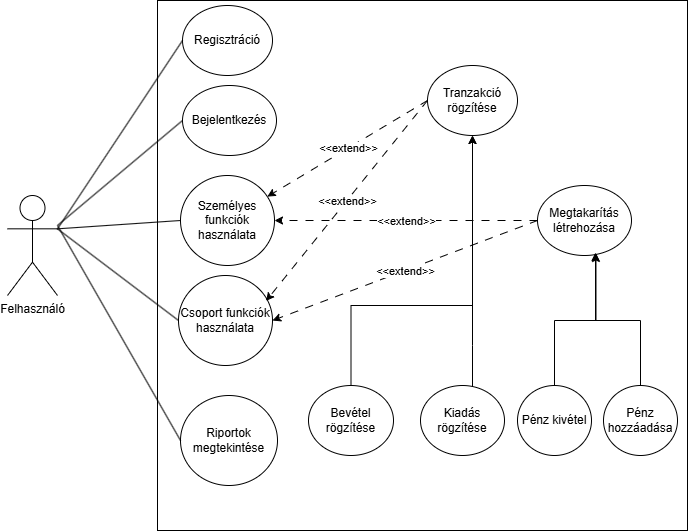
\includegraphics[height=220px]{img/big-use-case}
	\caption{Használati eset diagram: Általános}
	\label{fig:big-use-case}
\end{figure}

\subsection{Fiók}
A felhasználói fiókok kezelése a szokásos Regisztráció – Bejelentkezés – Profil funkciókra épül. A felhasználónak a webalkalmazás elérése érdekében regisztrálnia kell, majd sikeres regisztrációt követően bejelentkezhet a felületre. A belső oldalra érve elérhető egy "Profil" oldal a bal menüsávból is, illetve a jobb felső sarokban az avatar ikonra kattintva a legördülő menüből is kiválasztható ez a menüpont. Szintén ezen a két helyen találjuk a kijelentkezés gombot is, amellyel megszüntethetjük az adott munkamenetet és kiléphetünk a fiókból. Ezen funkciók részletes leírását a \ref{tab:account}. táblázat foglalja össze.
\subsubsection{Fiók kezelés}

\begin{table}[H]
	\centering
	\begin{tabular}{ | m{0.25\textwidth} | m{0.65\textwidth} | }
		\hline
		\textbf{Funkció} & \textbf{Leírás} \\
		\hline \hline
		\emph{Bejelentkezés} & Bejelentkezés egy egyedi felhasználónévvel és egy jelszóval lehetséges. (\ref{fig:login}. ábra) \\
		\hline
		\emph{Regisztráció} &  Regisztrálni lehet az oldalra a következő adatok megadásával: e-mail cím, felhasználónév (egyedi), teljes név, jelszó. Jelszó kritériumok: legalább 8 karakter, nagybetűt, kisbetűt, számot és egy speciális karaktert is tartalmaznia kell. (\ref{fig:register}. ábra)  \\
		\hline
		\emph{Profil} & A Profil oldalon lehet a fiókhoz tartozó adatokat módosítani: a felhasználónevet, a teljes nevet, illetve az e-mail címet is. Itt elérhető még egy "Change Pass" gomb is, amely elnavigálja a felhasználót a jelszó megváltoztató felületre. A profil oldal használatát a \ref{tab:profile}. táblázat fejti ki bővebben. (\ref{fig:profile}. ábra) \\
		\hline
		\emph{Jelszó módosítás} & A Profil oldalról lehet a jelszó változtató felületet elérni a "Change Pass" gomb megnyomásával. Itt meg kell adni a következő adatokat: régi jelszó, új jelszó, új jelszó megerősítése. \\
		\hline
		\emph{Kijelentkezés} & Ha a felhasználó befejezte kívánt tevékenységét, akkor a bal oldali menüsáv alján található "Logout" gomb megnyomásával tud kijelentkezni. A kijelentkező gomb még elérhető a jobb felső sarokban található ember ikonra kattintva legördülő menüben is. \\
		\hline
	\end{tabular}
	\caption{Fiók műveletek}
	\label{tab:account}
\end{table}

\begin{figure}[H]
	\centering
	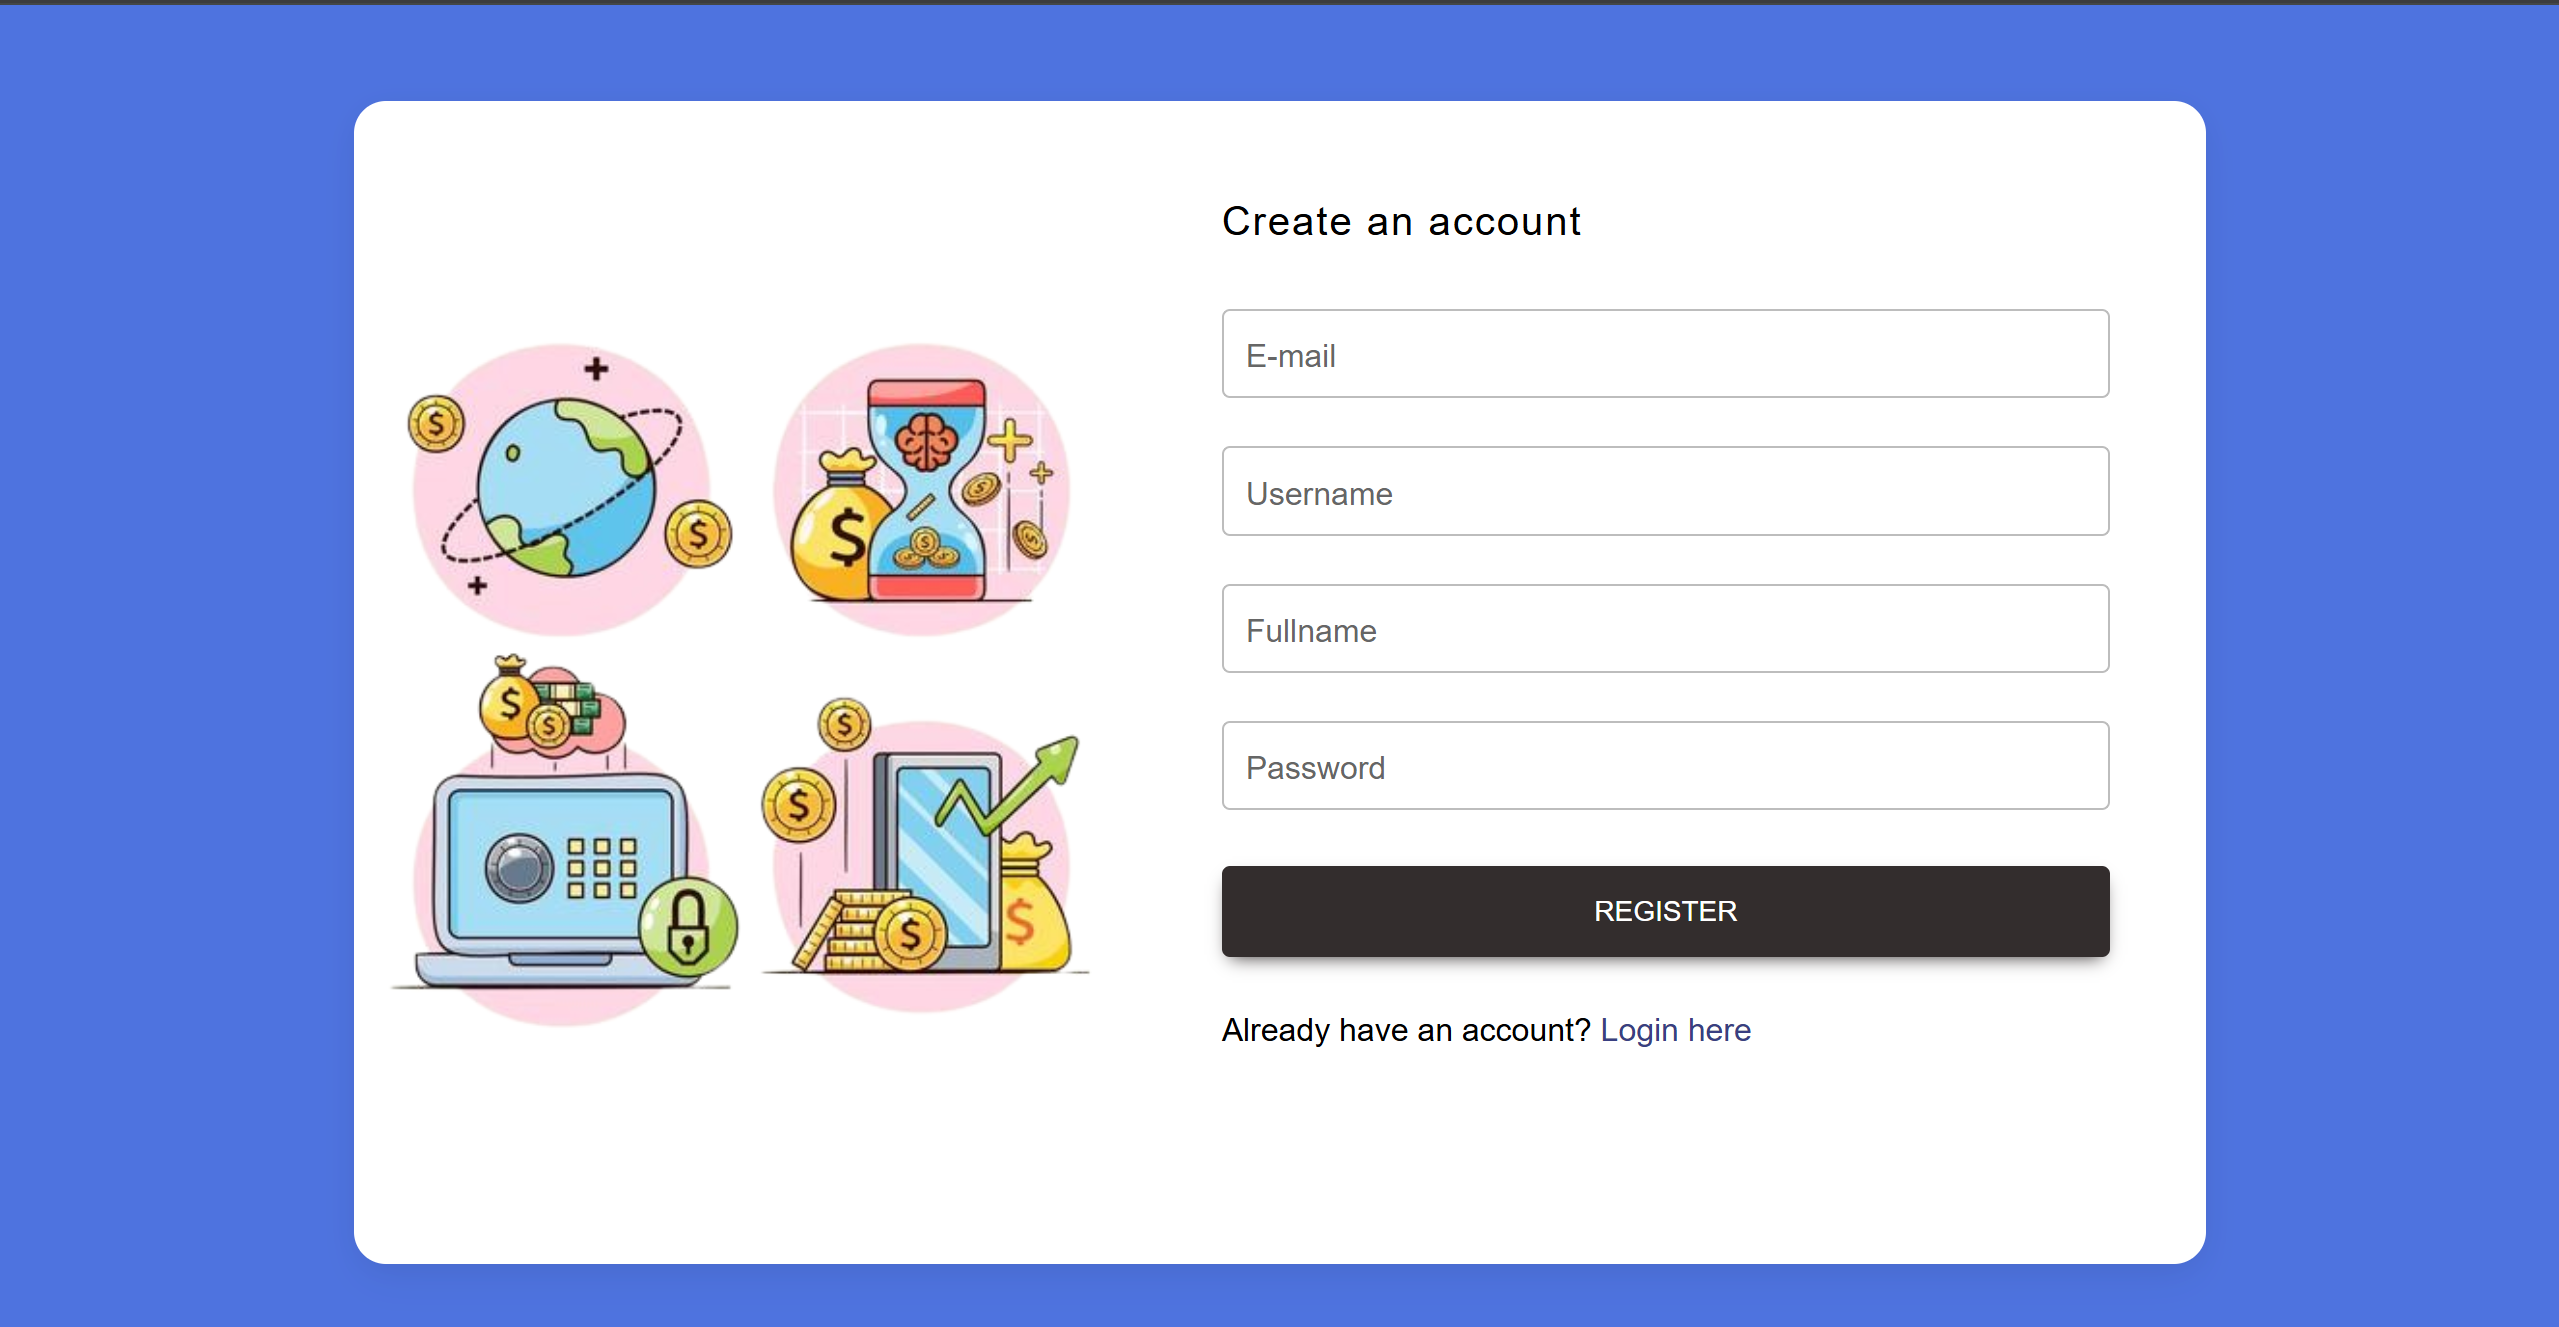
\includegraphics[height=160px]{img/register}
	\caption{Screenshot: Regisztrációs felület}
	\label{fig:register}
\end{figure}

\begin{figure}[H]
	\centering
	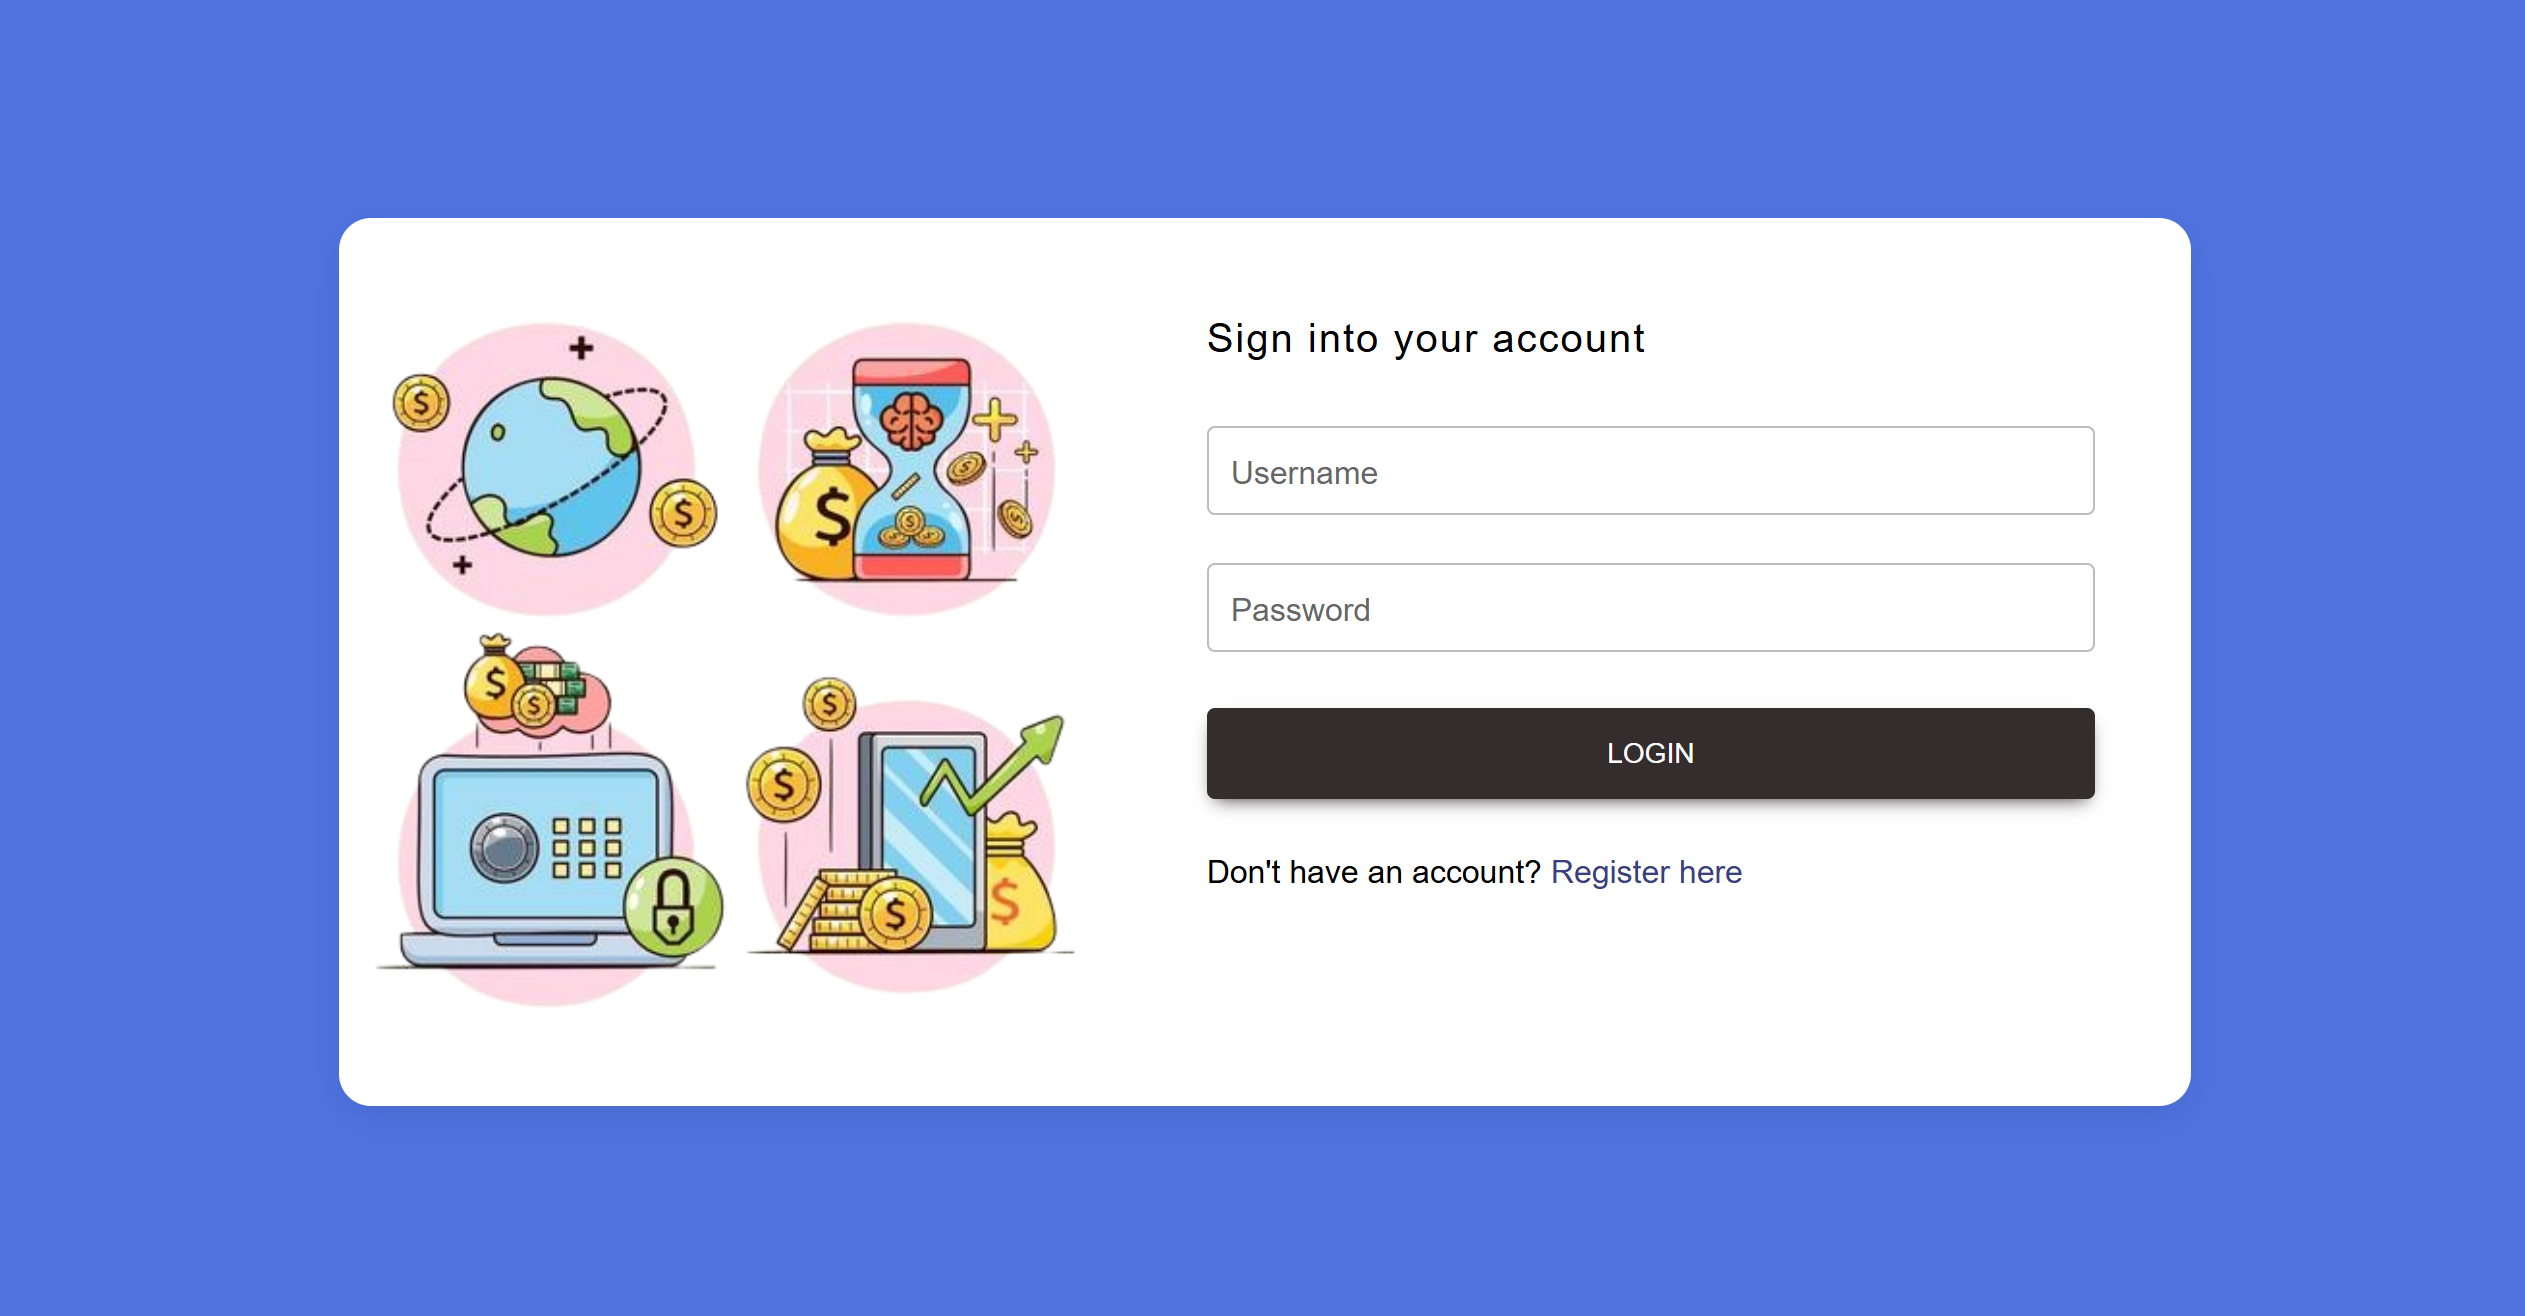
\includegraphics[height=150px]{img/login}
	\caption{Screenshot: Bejelentkező felület}
	\label{fig:login}
\end{figure}

\subsubsection{Profil}
\begin{table}[H]
	\centering
	\begin{tabular}{ | m{0.25\textwidth} | m{0.65\textwidth} | }
		\hline
		\textbf{Funkció} & \textbf{Leírás} \\
		\hline \hline
		\emph{Adatok megtekintése} & A regisztrációnál megadott személyes adatait a felhasználó itt tekintheti meg. \\
		\hline
		\emph{Adatok módosítása} &  A személyes adatok módosítására is itt van lehetőség, egyszerű beviteli mezőkkel lehet módosítani a felhasználónevet (egyedi), teljes nevet és e-mail címet. A "Change" gombra kattintva előugrik egy beviteli mező egy "Save" és "Cancel" gombbal kiegészítve. Az előbbi megpróbálja végrehajtani a kért módosítást, és jelzi az esetlegesen fellépő hibát (érvénytelen e-mail cím, foglalt felhasználónév, stb.) a felhasználó felé.  \\
		\hline
		\emph{Jelszó módosítás} & Ha a felhasználó módosítani kívánja a jelszavát, akkor a "Change Password" gombra kattintva megjelenik egy új felület, három jelszó beviteli mezővel (régi, új, új megerősítése). Jelszó kritériumok: legalább 8 karakter, nagybetűt, kisbetűt, számot és egy speciális karaktert is tartalmaznia kell. \\
		\hline
	\end{tabular}
	\caption{Profil oldal}
	\label{tab:profile}
\end{table}

\begin{figure}[H]
	\centering
	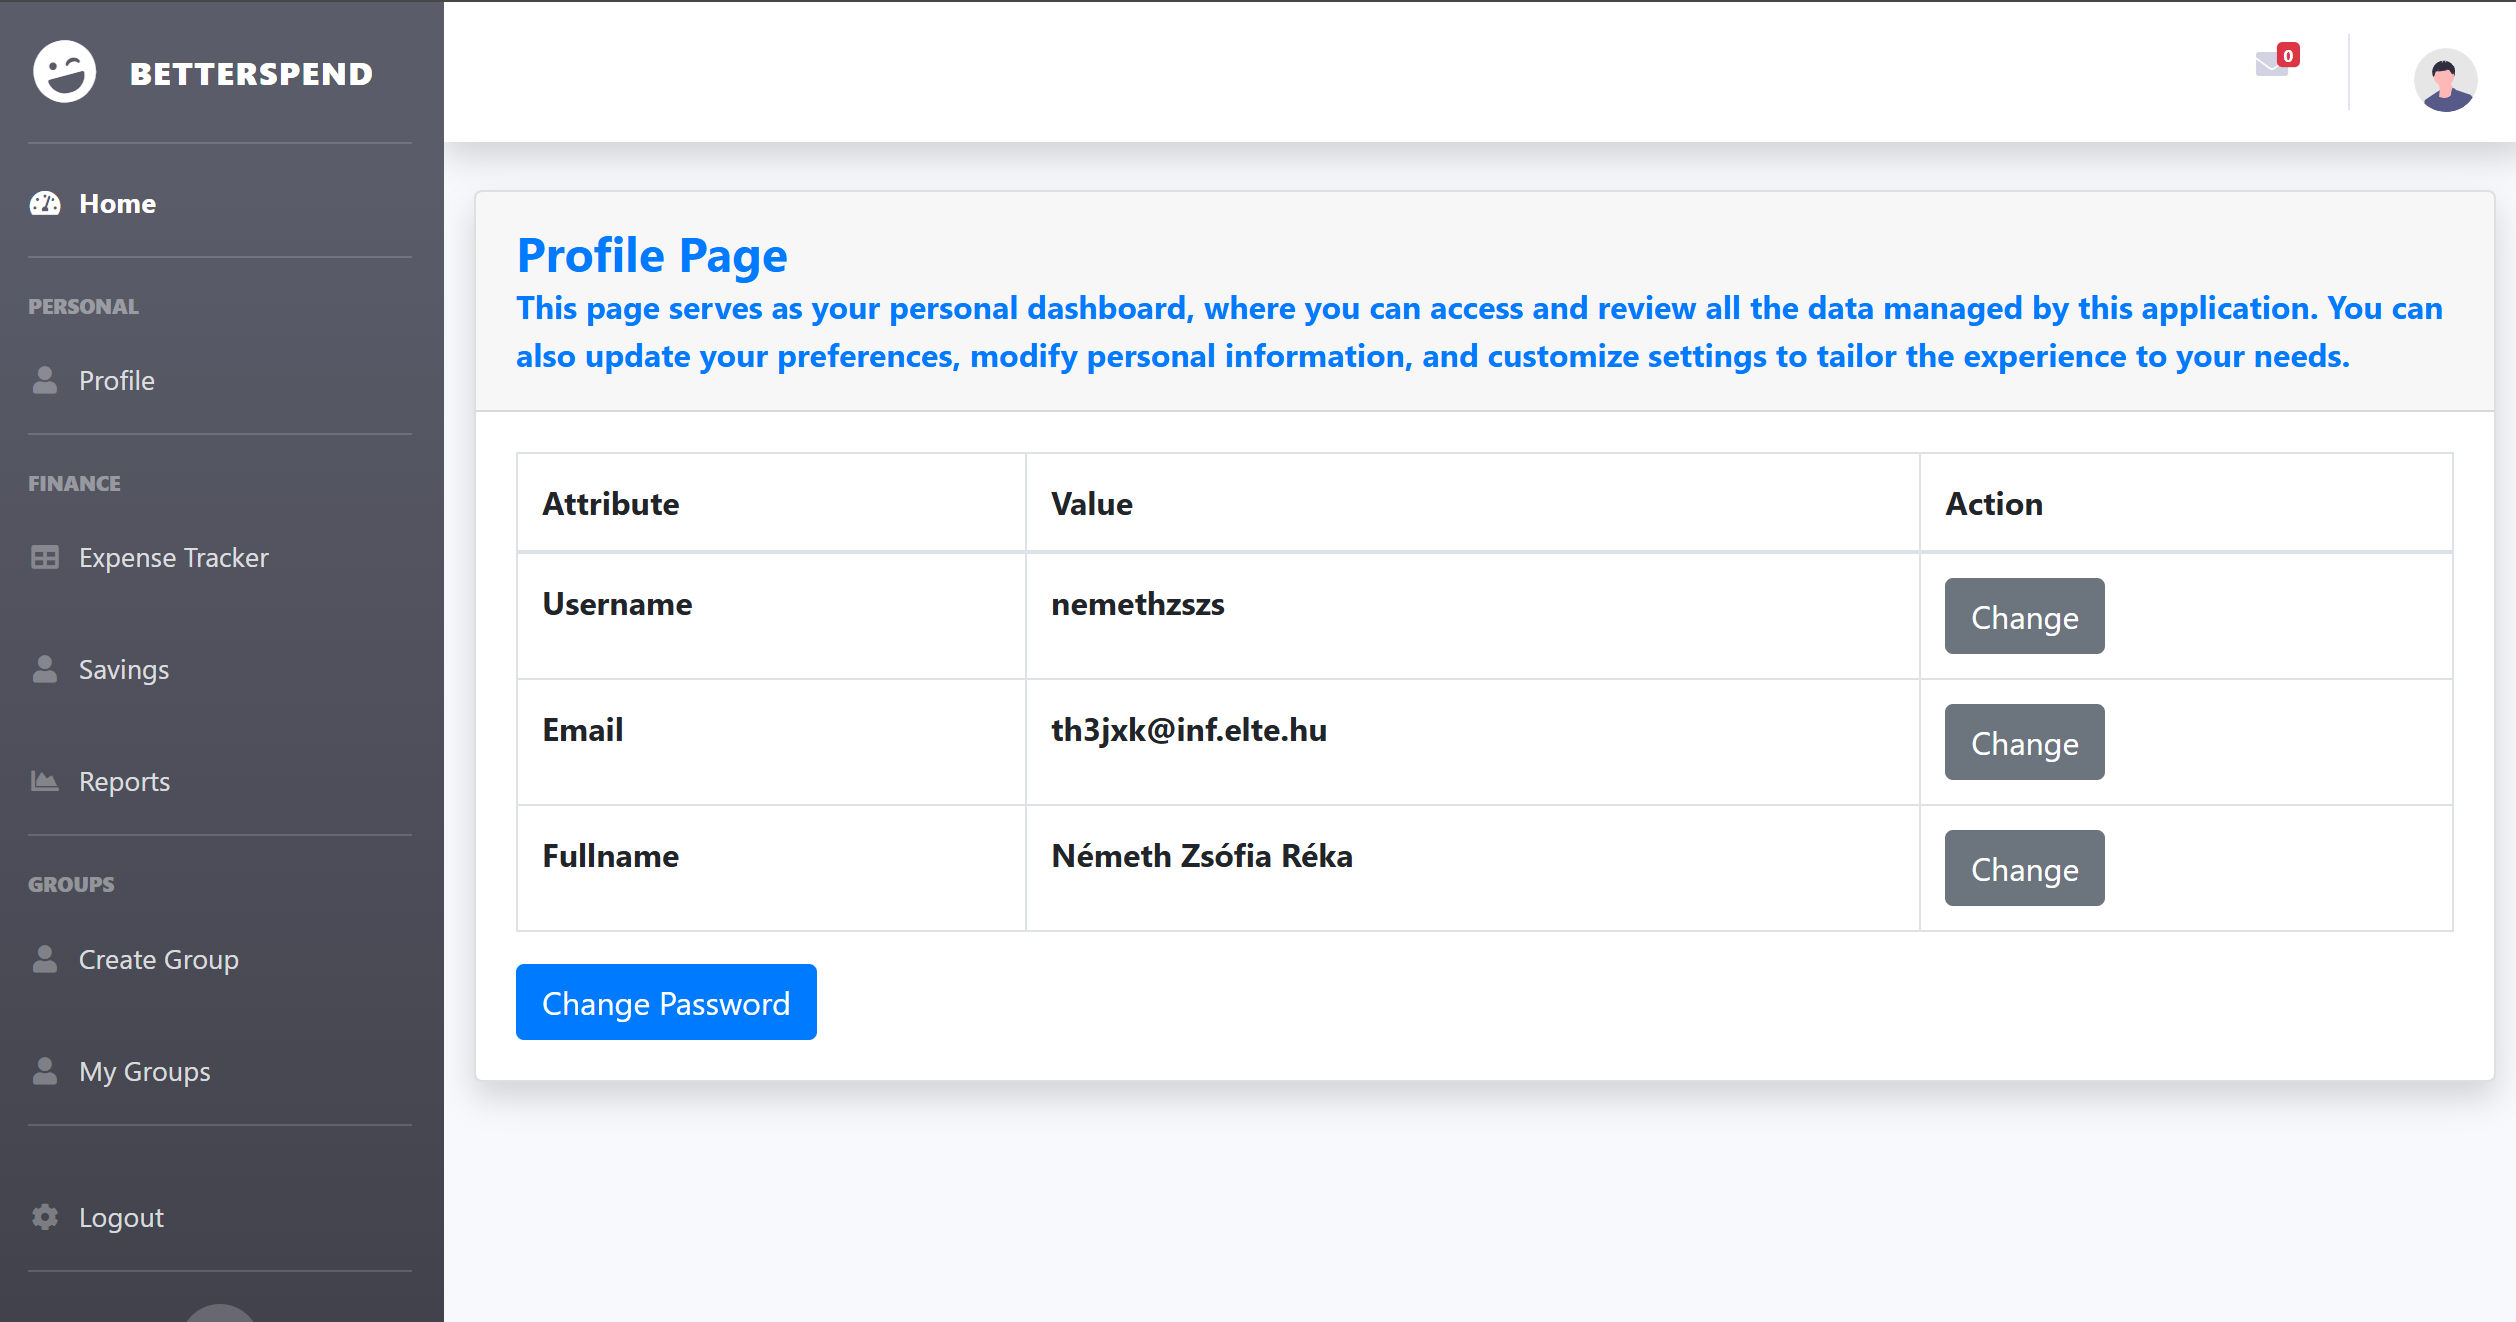
\includegraphics[height=150px]{img/profile}
	\caption{Screenshot: Profil felület}
	\label{fig:profile}
\end{figure}

\subsection{Pénzügyek}
A pénzügyeket kezelő oldalakat a kezdőképernyőről, illetve a baloldalon lévő menüből érhetjük el. A "Finance" cím alatt 3 különböző lap került kialakításra.
\begin{itemize}
	\item Tracker - Bevételek és kiadások vezetése, havi költési limit kezelése és előzmények megtekintése
	\item Savings - Megtakarítások megtekintése és kezelése
	\item Reports - Kimutatások megtekintése, személyre szabása és exportálása
\end{itemize}

\subsubsection{Tracker felület}
A Tracker felület foglalja magában a bevételek és kiadások vezetését, havi költési limit módosítását és monitorozását, illetve az előzmények megtekintését és korábbi tranzakciók eltávolítását. Az oldal 3 különböző lapból áll, ezek között lehet navigálni az oldal tetején lévő gombok segítségével (\ref{fig:tracker-tabs}. ábra).
\begin{figure}[H]
	\centering
	
\includegraphics[height=40px]{img/tracker-tabs}
	\caption{Screenshot: Tracker felület navigációs sáv}
	\label{fig:tracker-tabs}
\end{figure}
\begin{itemize}
	\item Transactions (\ref{tab:transactions}. táblázat és \ref{fig:transactions}. ábra) (Bevételek és kiadások vezetése, és előzmények megtekintése)
	\item Batch Upload (\ref{tab:batch-upload}. táblázat és \ref{fig:batch-upload}. ábra) (Tömeges bejegyzés-feltöltés)
	\item Monthly Spending Limit (\ref{tab:monthly-limit}. táblázat és \ref{fig:monthly-limit}. ábra) (Költési limit kezelése) 
\end{itemize}

\pagebreak
\begin{itemize}
	\item[\emph{Transactions}]
	A tranzakciókkal kapcsolatos funkciók leírását a \ref{tab:transactions}. táblázat tartalmazza.
	\begin{table}[H]
		\centering
		\begin{tabular}{ | m{0.25\textwidth} | m{0.65\textwidth} | }
			\hline
			\textbf{Funkció} & \textbf{Leírás} \\
			\hline \hline
			\emph{Kiadás/bevétel rögzítése} & Külön dobozokban lehet rögzíteni a kiadásokat, és a bevételeket. Egyszerre egyet lehet bevinni, melynek adni kell egy összeget, egy leírást, opcionálisan lehet kategóriát is megadni. Ha kiadást rögzítünk, akkor egy felugró ablak jelzi minden alkalommal, hogy mennyi maradt még a havi költési limitből, illetve ha már túl lett lépve, akkor egy figyelmeztető ablak ugrik fel. \\
			\hline
			\emph{Előzmények} &  A költési és bevételi előzményeket is itt lehet megtekinteni egy összesítő táblázatban. A táblázatban felül a "Search" mező módosításával lehet szűrni címszó alapján, azaz tudunk bármire (összegre, címre, kategóriára, stb.) keresni. Illetve az oszlopok címeire kattintva rendezni is lehet őket. A táblázat utolsó ("Delete") oszlopa arra szolgál, hogy egy adott sorban a kuka ikonra rákattintva, az a bejegyzés törlődik.  \\
			\hline
		\end{tabular}
		\caption{Transactions lap}
		\label{tab:transactions}
	\end{table}
	\begin{figure}[H]
		\centering
		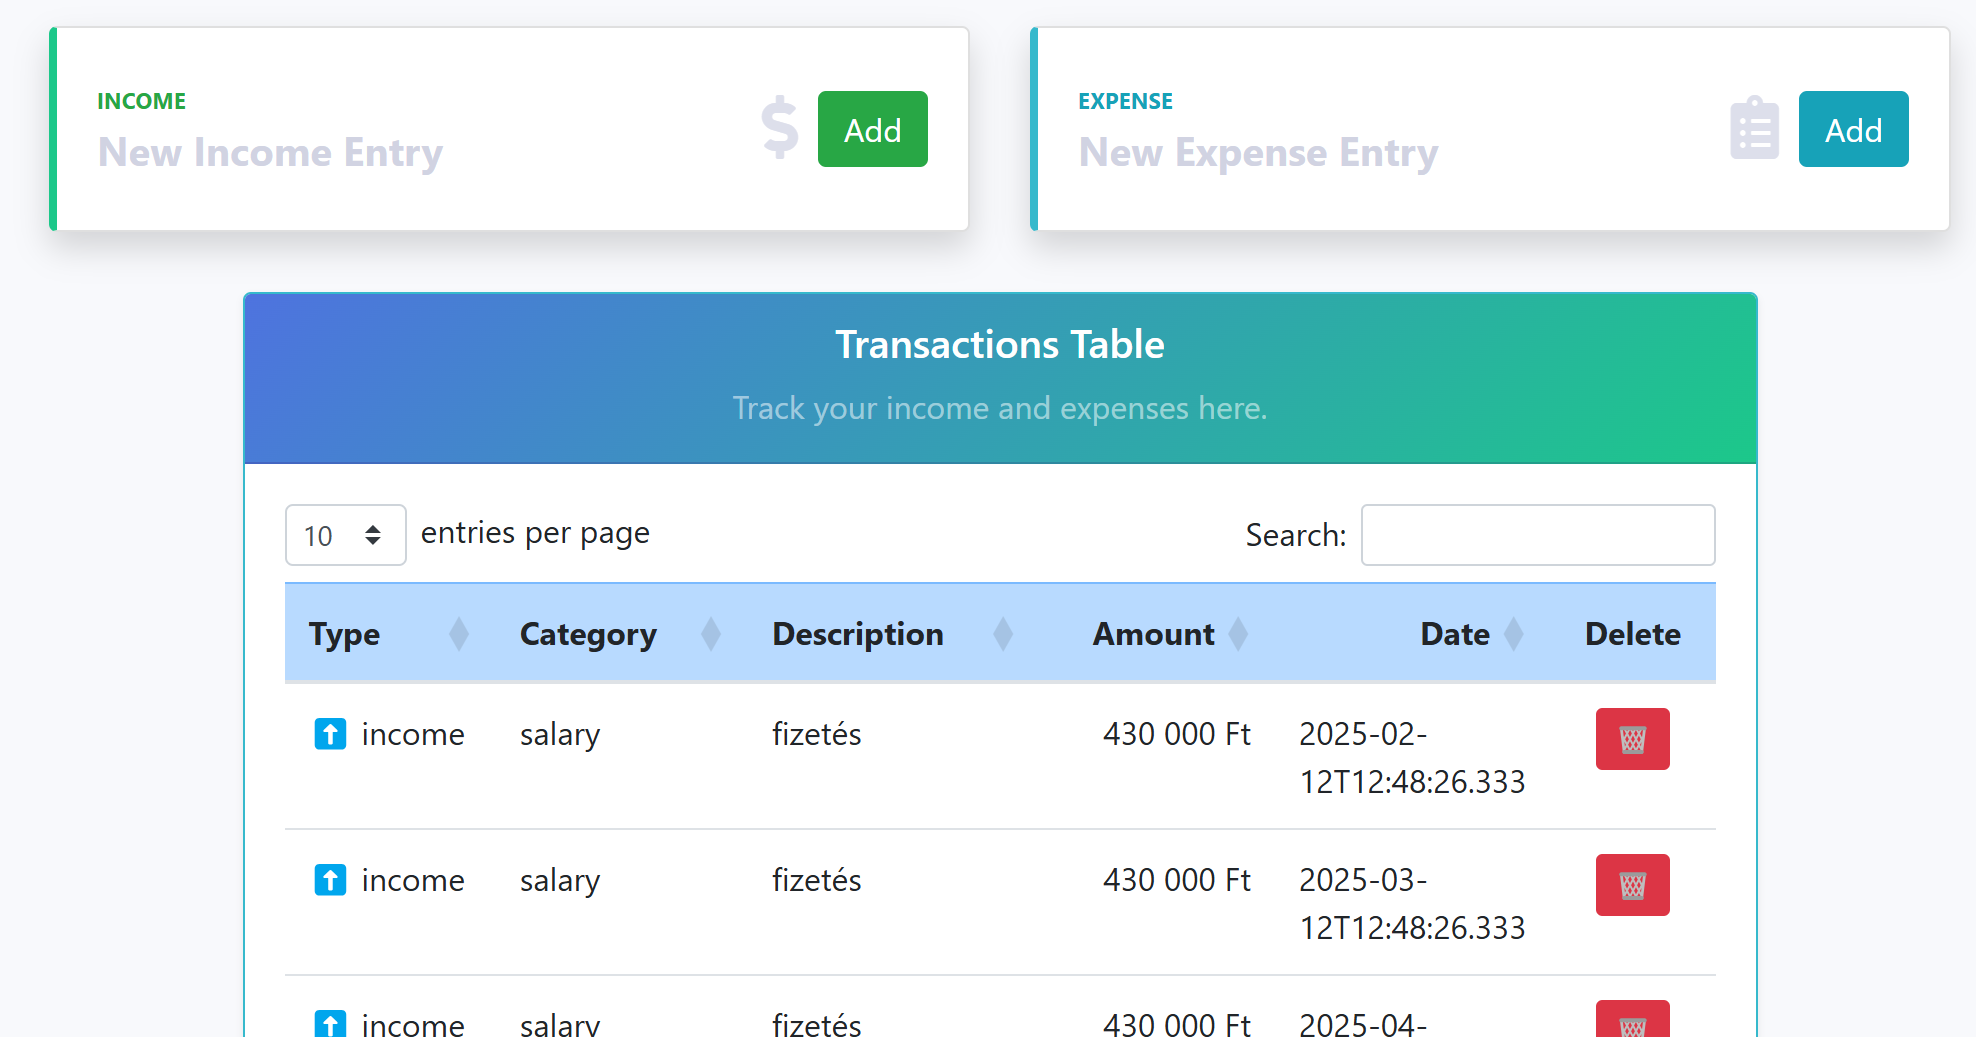
\includegraphics[height=180px]{img/transactions}
		\caption{Screenshot: Transactions lap}
		\label{fig:transactions}
	\end{figure}
	\pagebreak
	\item[\emph{Batch Upload}] 
	A tömeges feltöltéssel kapcsolatos funkciókat a \ref{tab:batch-upload}. táblázat tartalmazza.
	\begin{table}[H]
		\centering
		\begin{tabular}{ | m{0.25\textwidth} | m{0.65\textwidth} | }
			\hline
			\textbf{Funkció} & \textbf{Leírás} \\
			\hline \hline
			\emph{CSV feltöltés} & A felhasználó számára lehetőség adott tömeges tranzakció bejegyzés feltöltésére. Egy ("," vagy ";" karakterekkel tagolt) .csv kiterjesztésű fájl feltöltésével automatikusan rögzítésre kerülnek a benne szereplő tranzakciók. A fájl helyes felépítése a \ref{src:csv}. forráskód ábrán látható. Minden mező kitöltése kötelező, illetve kategóriából csak a felületen már létező kategória érték adható meg.  Az általános sor struktúra: [típus (1 = bevétel, 2 = kiadás), kategória (vagy "-" ha nem kívánja megadni), leírás, összeg (pozitív egész szám), dátum (formátum: YYYY-MM-DD)]\\
			\hline
		\end{tabular}
		\caption{Batch upload lap}
		\label{tab:batch-upload}
	\end{table}
	\lstset{caption={Tömeges feltöltés: csv fájl struktúra}, label=src:csv}
	\begin{lstlisting}[language={[Sharp]C}]
		2, family, vacsi petivel, 10500, 2024-10-12
		2, family, botanikus kert, 12300, 2024-11-15
		1, -, ruha, 4500, 2024-09-24 
	\end{lstlisting}
	
	\begin{figure}[H]
		\centering
		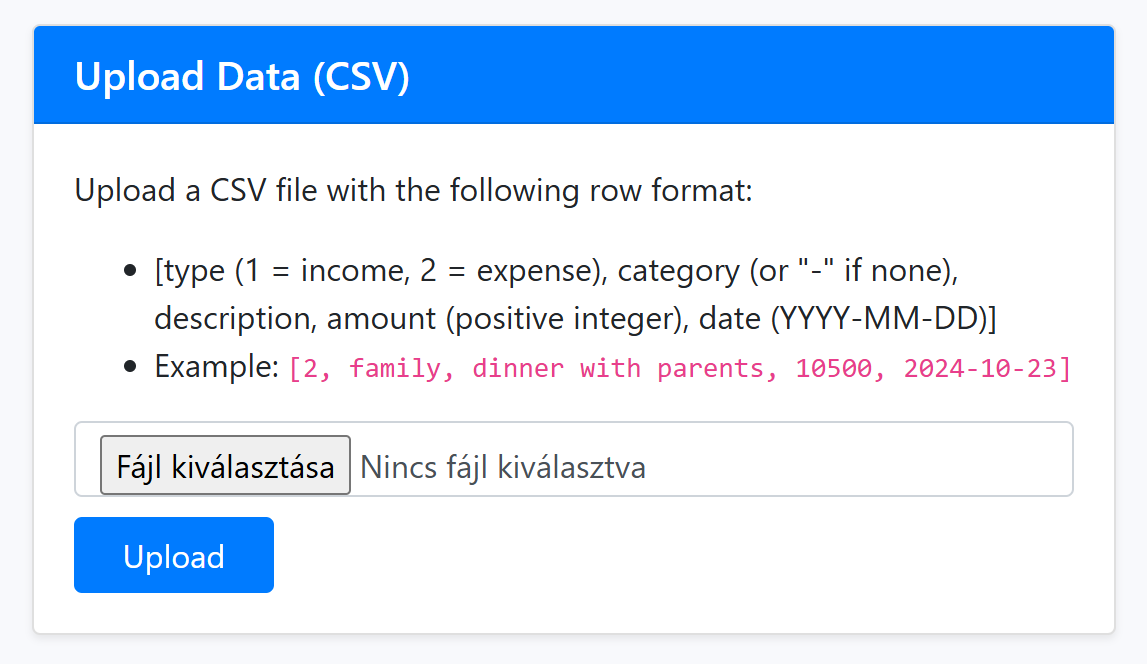
\includegraphics[height=180px]{img/batch-upload}
		\caption{Screenshot: Tömeges feltöltés lap}
		\label{fig:batch-upload}
	\end{figure}
	\pagebreak
	\item[\emph{Spending Limit}]
	A havi költési limittel kapcsolatos funkciók leírását a \ref{tab:monthly-limit}. táblázat tartalmazza.
	\begin{table}[H]
		\centering
		\begin{tabular}{ | m{0.25\textwidth} | m{0.65\textwidth} | }
			\hline
			\textbf{Funkció} & \textbf{Leírás} \\
			\hline \hline
			\emph{Havi költési limit módosítása} & Itt tudja a felhasználó a havi költési limitjét módosítani. A "Change" gombra kattintva előugrik egy beviteli mező és egy "Save" (mentés) gomb. \\
			\hline
			\emph{Diagram} &  A költési limit vizuális nyomon követését segíti a lapon elhelyezett kördiagram, amely egyszerű módon mutatja, hogy mennyit költött már a felhasználó a limitből. \\
			\hline
		\end{tabular}
		\caption{Monthly Spending limit lap}
		\label{tab:monthly-limit}
	\end{table}
	\begin{figure}[H]
		\centering
		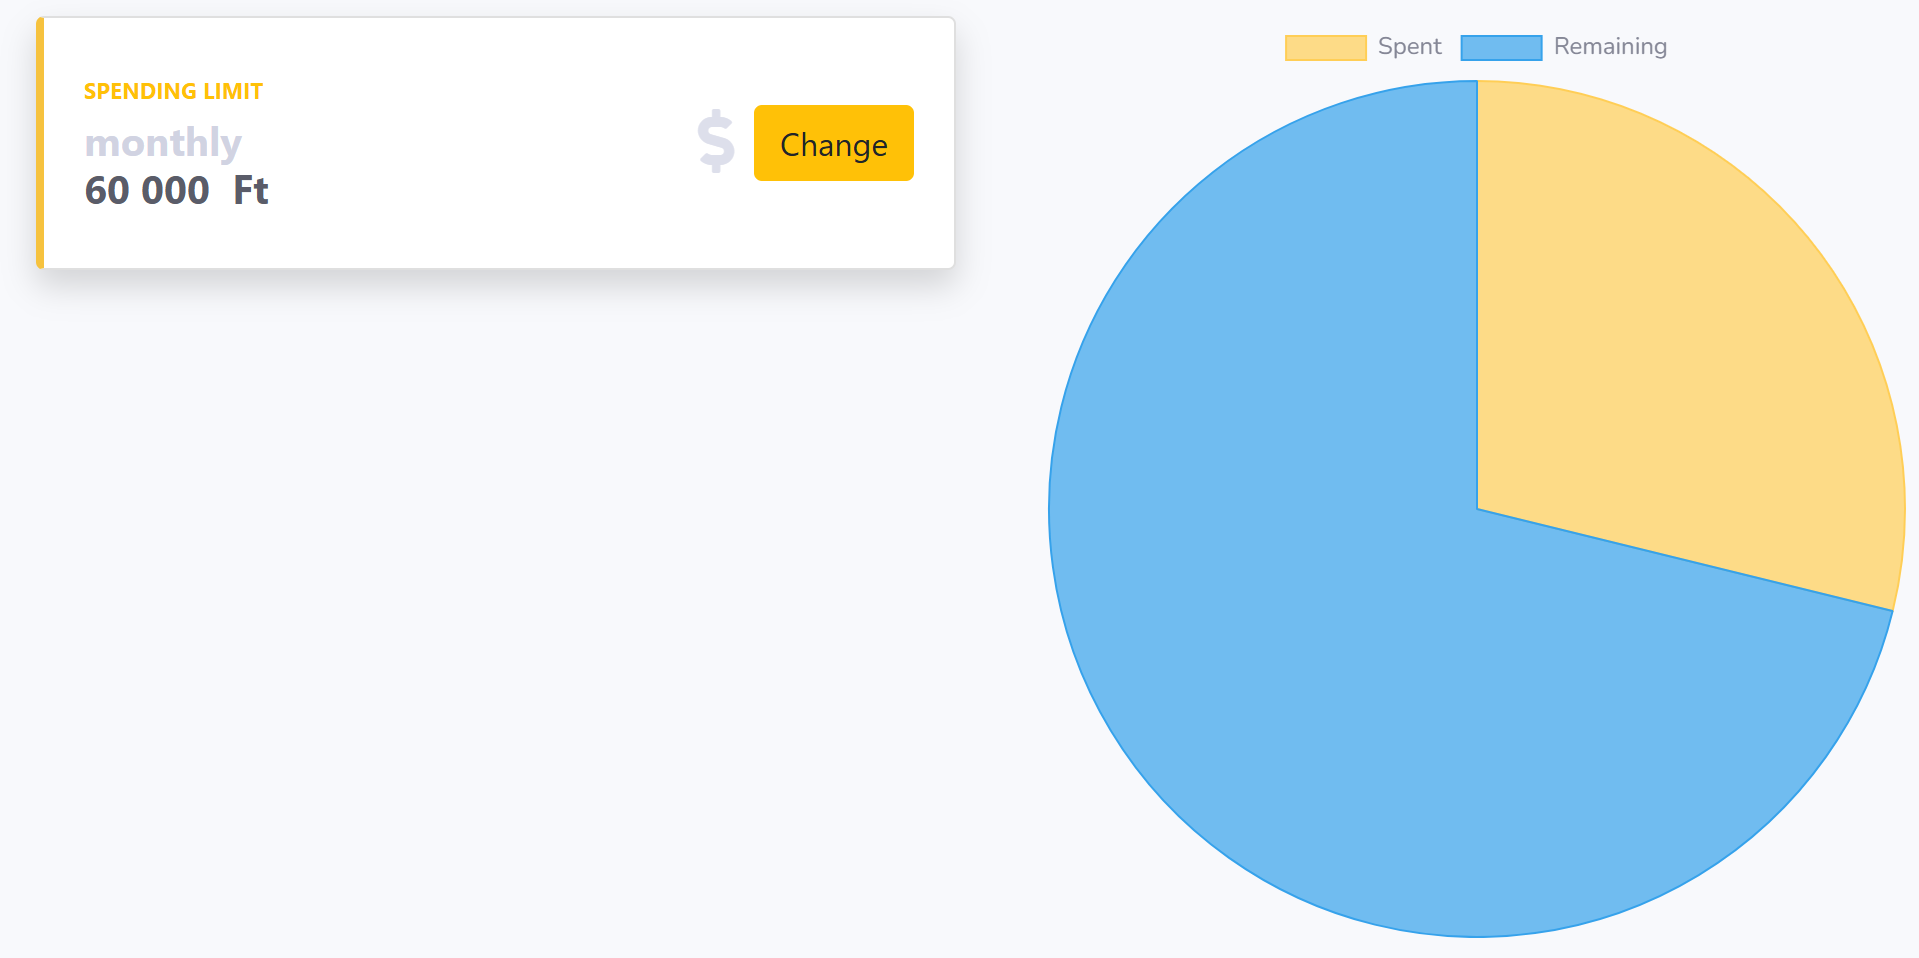
\includegraphics[height=180px]{img/monthly-limit}
		\caption{Screenshot: Monthly Spending Limit lap}
		\label{fig:monthly-limit}
	\end{figure}
\end{itemize}

\subsubsection{Megtakarítás felület}
\begin{itemize}
	\item[\emph{Gyűjtés létrehozása}] 
	A felhasználó új megtakarítási célt hozhat létre, például egy konkrét vásárlás vagy vészhelyzeti alap létrehozásához. A cél tartalmazhat megnevezést, opcionális leírást, célösszeget és határidőt. A cél a főoldalon egy külön kártyaként jelenik meg. Egy új gyűjtést a \ref{fig:addsaving}. ábrán látható felület kitöltésével tud hozzáadni a felhasználó, amely az "Add new saving goal" gomb megnyomásával ugrik fel.
	\begin{figure}[H]
		\centering
		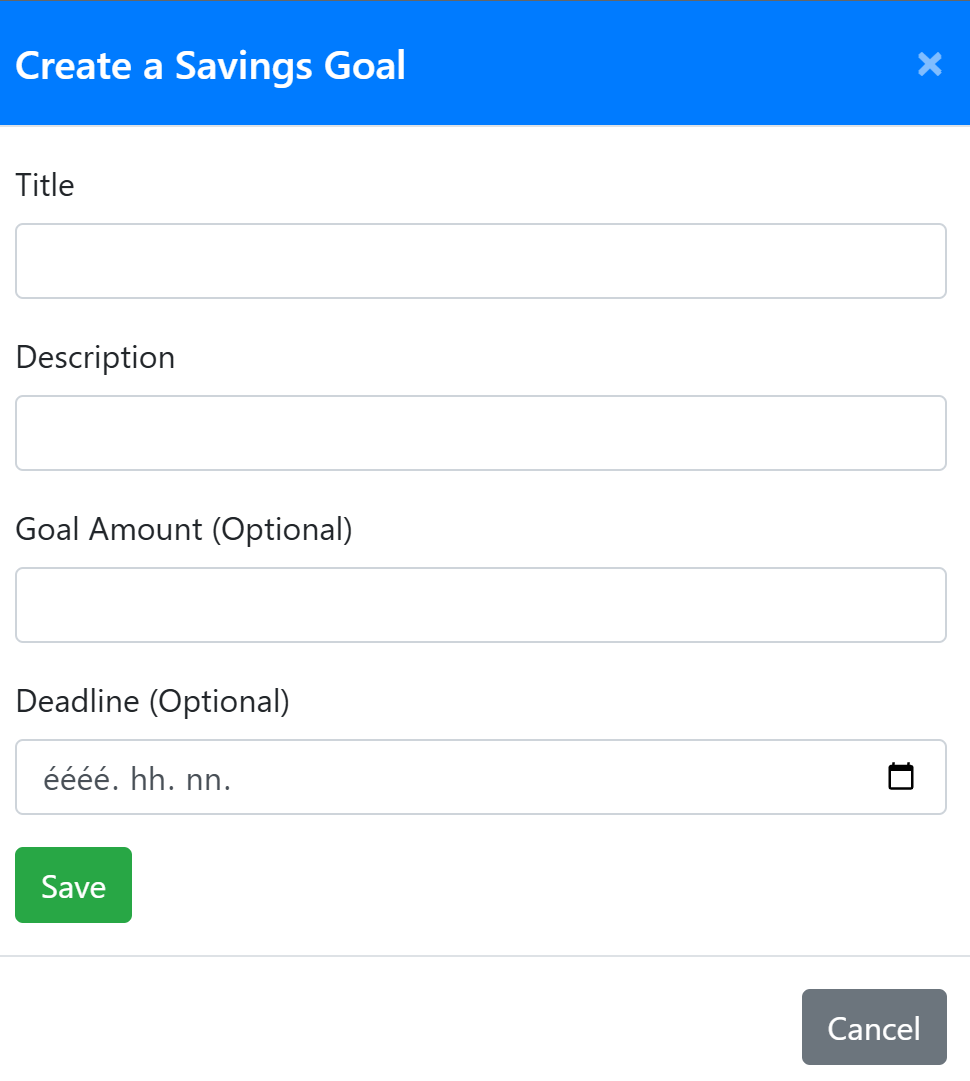
\includegraphics[height=190px]{img/add-saving}
		\caption{Screenshot: Gyűjtés létrehozása}
		\label{fig:addsaving}
	\end{figure}
	\item[\emph{Gyűjtések kezelése}]
	A gyűjtéseket az egyes kártyákon belül elhelyezett gombok, és beviteli mezők segítségével lehet kezelni. Ezeket a funkciókat a \ref{tab:savings}. táblázat.
	\begin{table}[H]
		\centering
		\begin{tabular}{ | m{0.25\textwidth} | m{0.65\textwidth} | }
			\hline
			\textbf{Funkció} & \textbf{Leírás} \\
			\hline \hline
			
			\emph{Összeg hozzáadása a gyűjtéshez} &
			Lehetővé teszi, hogy a felhasználó megtakarított összeget adjon hozzá egy kiválasztott célhoz. A kártyán található beviteli mező és "Add to Savings" gomb segítségével történik a művelet. Az aktuális megtakarítás értéke és a haladás százalékos formában is megjelenik. \\
			
			\hline
			
			\emph{Összeg kivonása a gyűjtésből} &
			Amennyiben a felhasználó el kíván távolítani egy összeget a gyűjtésből (pl. téves bevitel miatt), azt megteheti a "Withdraw" gomb segítségével. Ez a funkció csökkenti a gyűjtött összeget, de nem törli a célt. \\
			
			\hline
			
			\emph{Gyűjtés törlése} &
			A gyűjtés jobb felső sarkában elhelyezett kuka ikon segítségével a felhasználó teljesen eltávolíthat egy megtakarítási célt. Ez véglegesen törli az adott kártyát és a hozzá tartozó adatokat. \\
			
			\hline
			
			\emph{Cél elérése vizualizáció} &
			Ha a megtakarított összeg eléri vagy meghaladja a kitűzött célt, a kártya vizuálisan zöld színre vált. \\
			
			\hline
		\end{tabular}
		\caption{A Savings oldal}
		\label{tab:savings}
	\end{table}
	\begin{figure}[H]
		\centering
		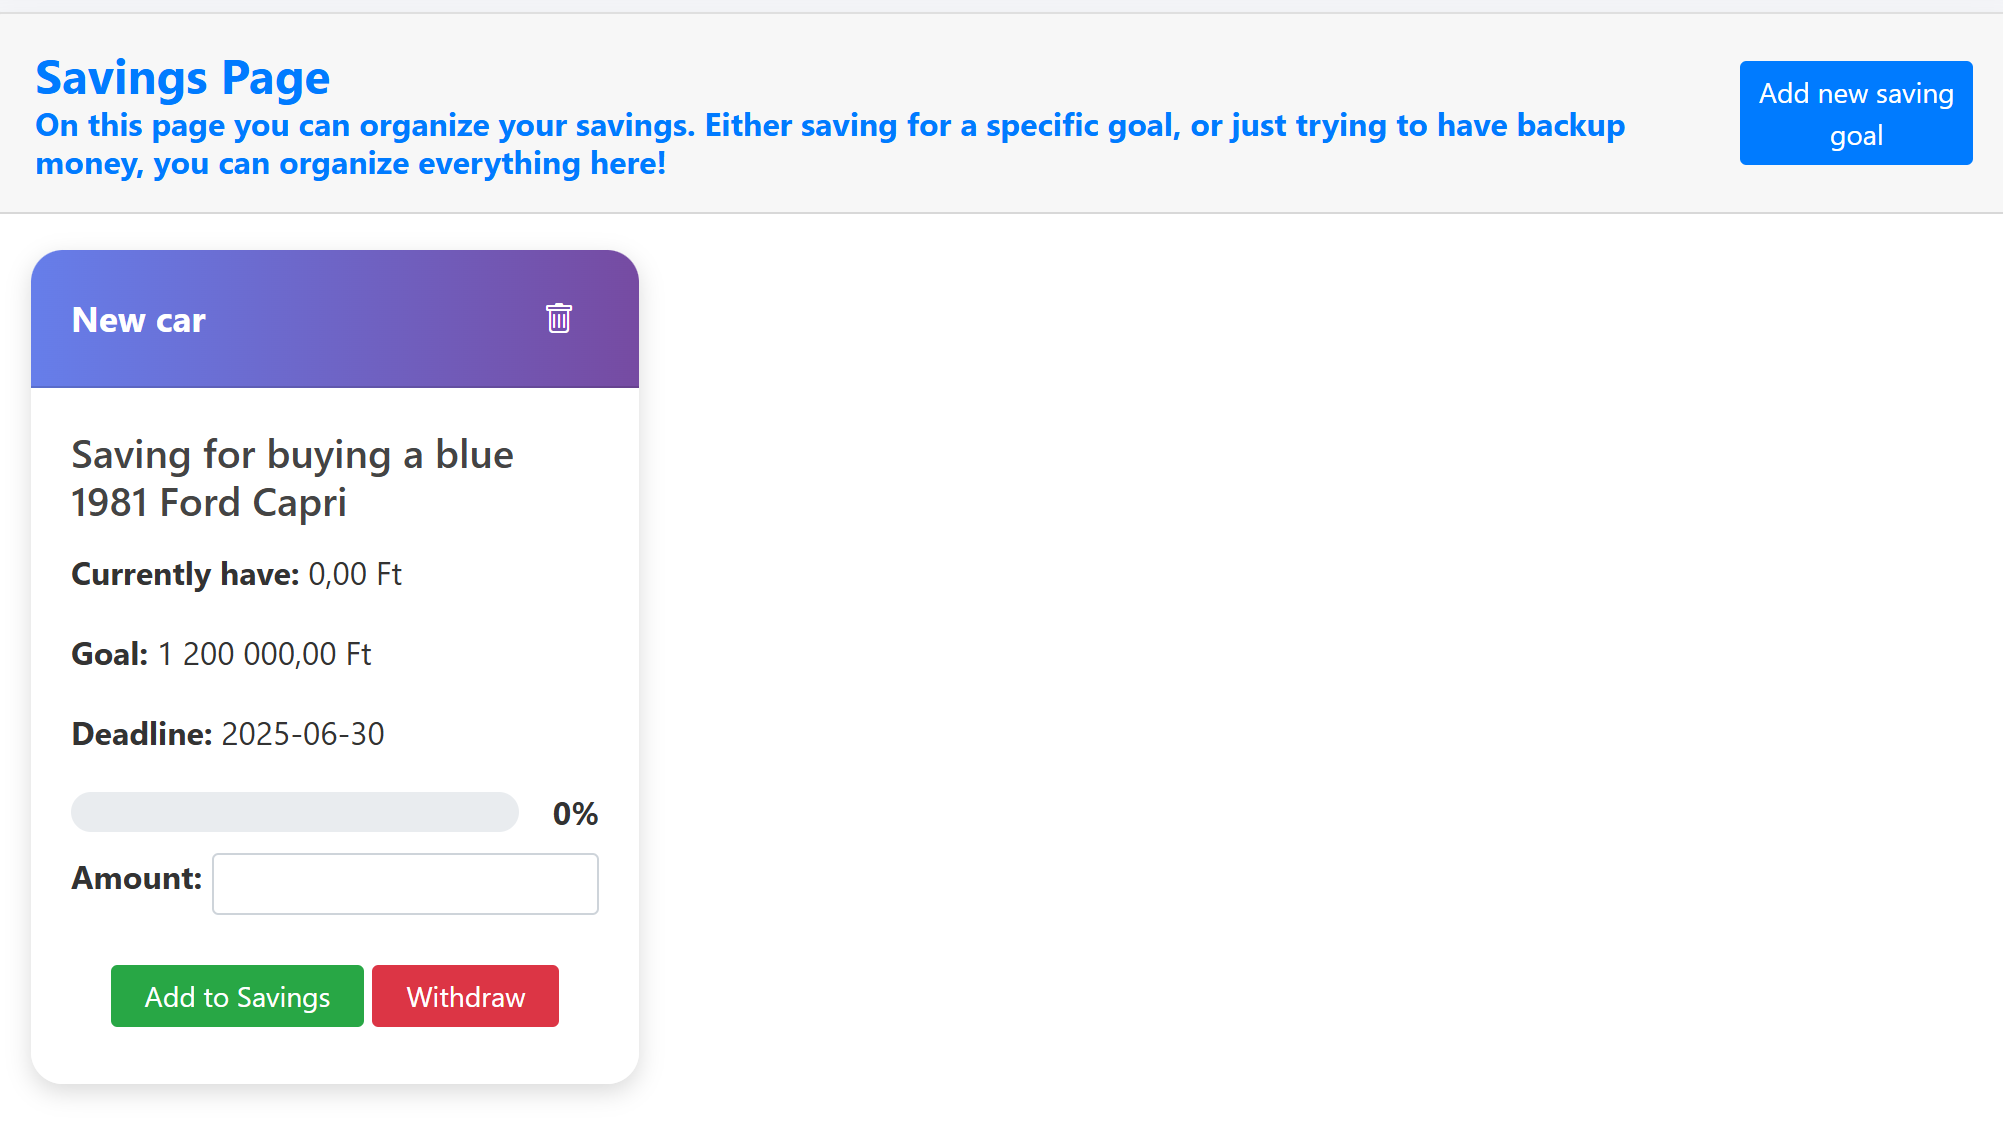
\includegraphics[height=190px]{img/savings}
		\caption{Screenshot: Savings felület}
		\label{fig:savings}
	\end{figure}
\end{itemize}


\subsubsection{Kimutatások felület}
\begin{itemize}
	\item[\emph{Havi riport}] Az oldal első szekciója egy vonaldiagramot jelenít meg (\ref{fig:report1}. ábra), amely napi bontásban mutatja az adott hónap bevételeit és kiadásait. A diagram segít a felhasználónak átlátni a pénzmozgásokat, észrevenni a kiugró értékeket. A színek jól elkülönítik a bevételt (zöld) és a kiadást (piros).
	\begin{figure}[H]
		\centering
		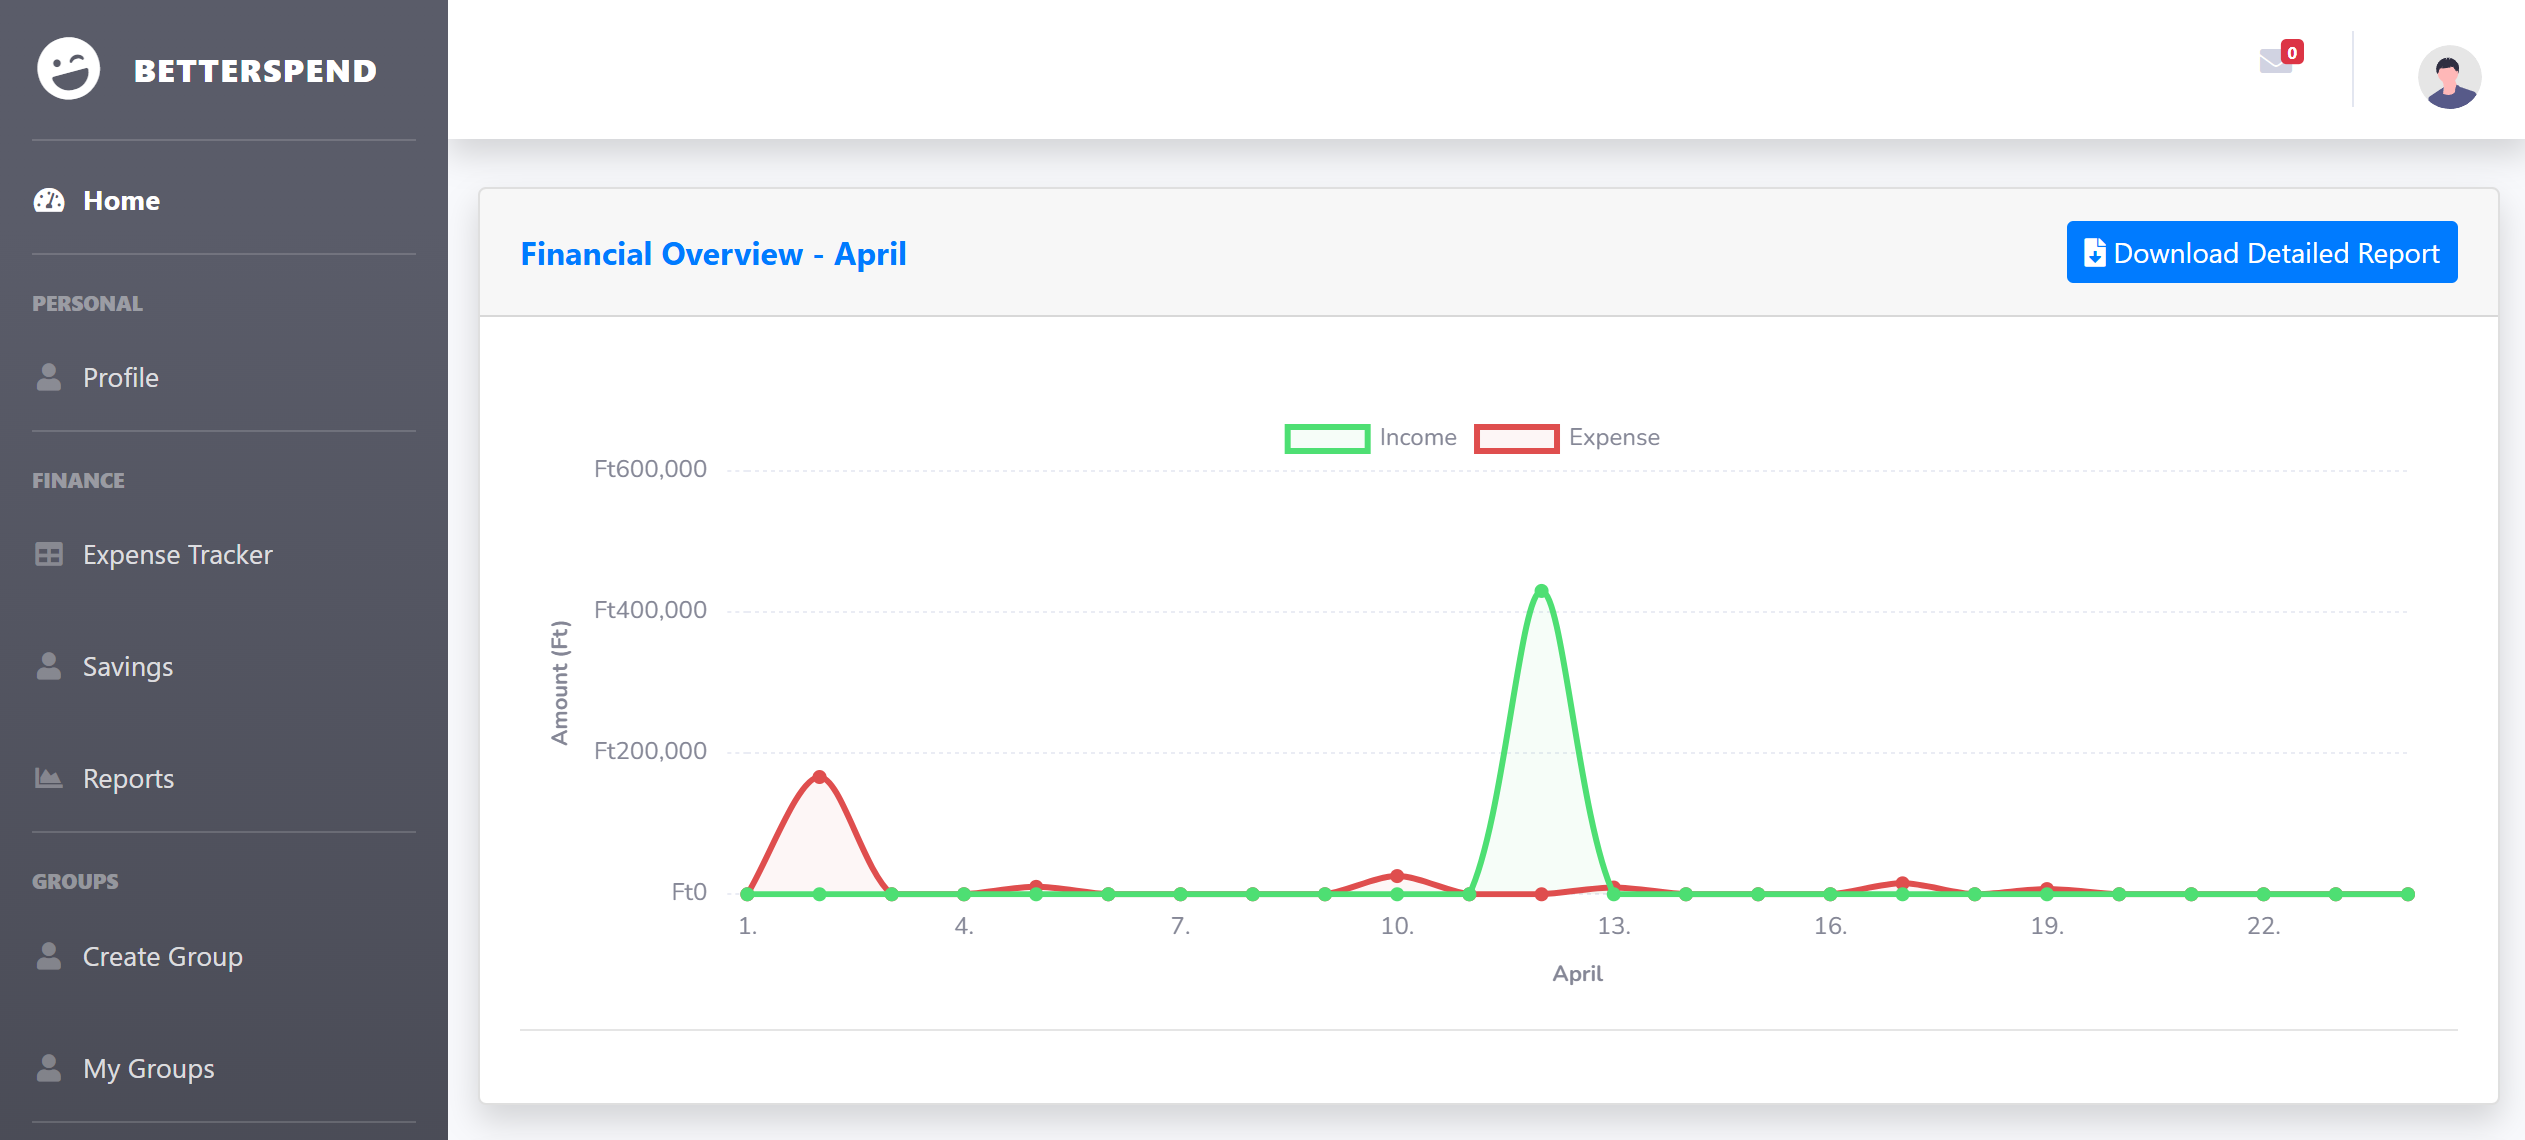
\includegraphics[height=190px]{img/reports1}
		\caption{Screenshot: Aktuális havi riport}
		\label{fig:report1}
	\end{figure}
	\item[\emph{Letöltés}] A "Download Detailed Report" gomb lehetőséget ad arra, hogy a felhasználó exportálja a részletes pénzügyi riportját az adott hónapra (PDF formátumban). Ez hasznos lehet adminisztrációhoz vagy hó végi összesítéshez.
	\item[\emph{Éves riport}] Egy oszlopdiagram (\ref{fig:report2}. ábra) összehasonlítja az egyes hónapok bevételi és kiadási értékeit. A felhasználó egy legördülő listából kiválaszthatja az évet (de alapértelmezetten az idei év adatai láthatóak), amely alapján frissül a diagram. Ez segít az éves pénzügyi trendek nyomon követésében.
	\begin{figure}[H]
		\centering
		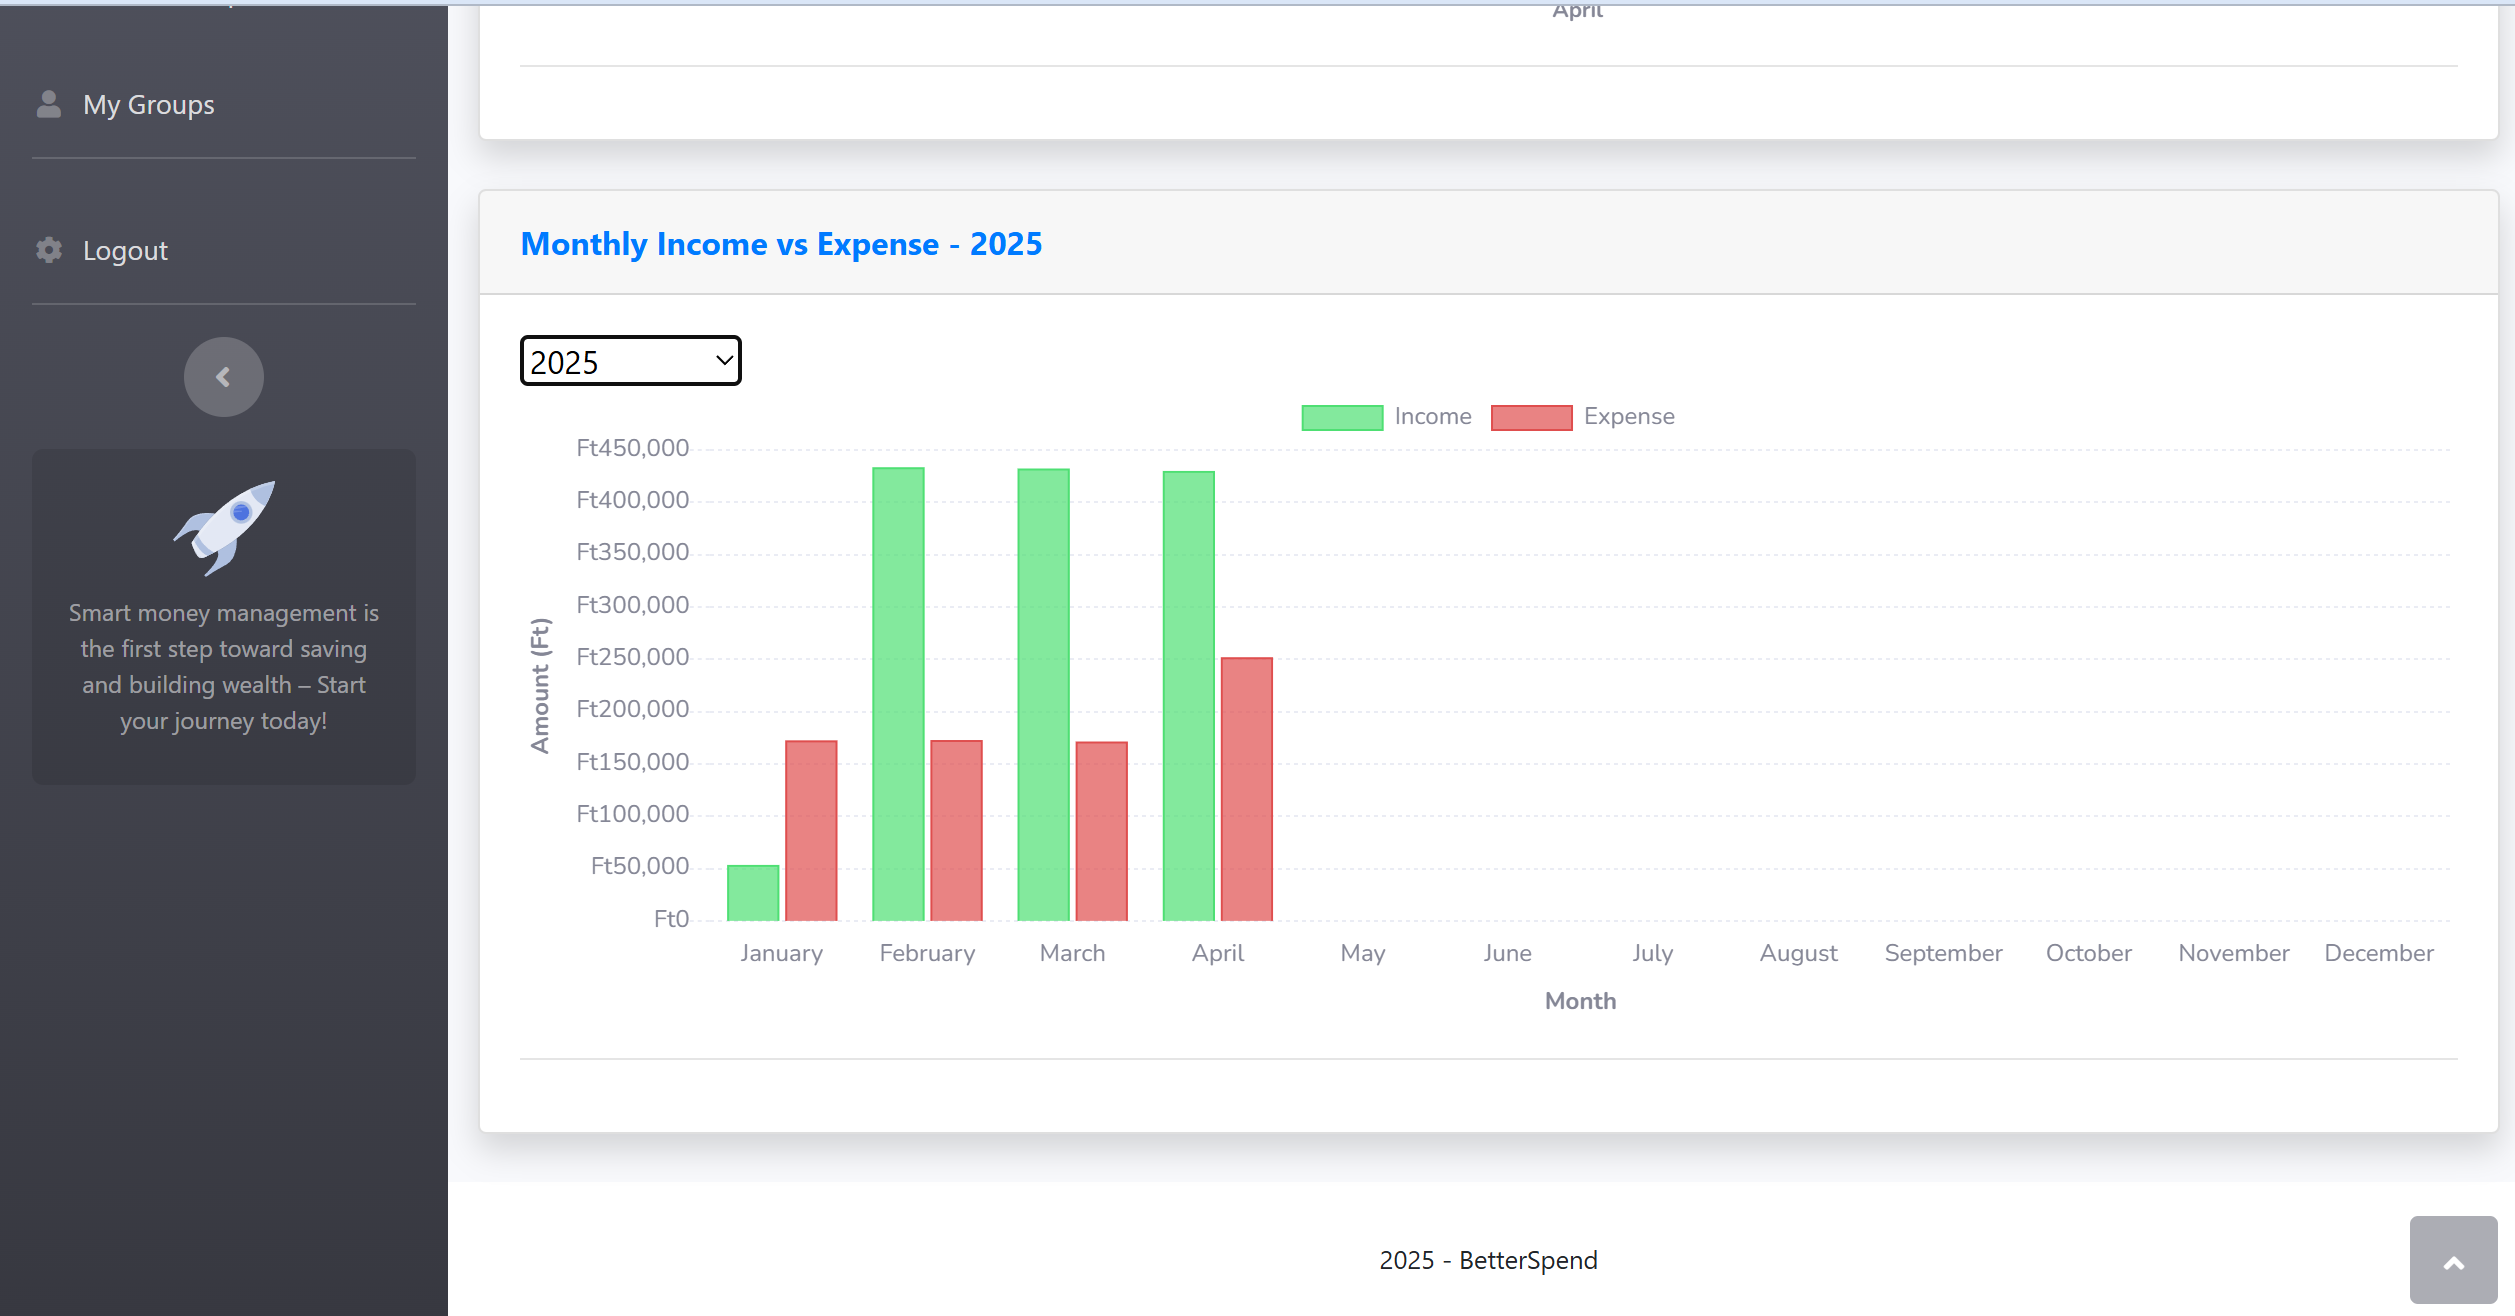
\includegraphics[height=190px]{img/reports2}
		\caption{Screenshot: Éves összesítő riport}
		\label{fig:report2}
	\end{figure}
\end{itemize}

\subsection{Csoportok}
A csoportokban valamennyi funkció elérhető, melyek a személyes használat esetében is. Ezeket az előző fejezetek taglalták részletesebben. A következő bekezdésben a csoportok kezelését és elérését fogom bemutatni.
\subsubsection{Csoport létrehozása}
Az \ref{fig:create-group}. ábrán látható felület a baloldali menüsávból érhető el ("Create Group" menüpont). Itt a következő adatok megadása szükséges: Title (csoport neve), Type (csoport típusa, ez csak a felhasználó számára egy rendszerezési lehetőség, jelentősége nincsen), Description (csoport részletesebb leírása). Ezután a "Create Group" gombra kattintva már kész is a csoport.
\begin{figure}[H]
	\centering
	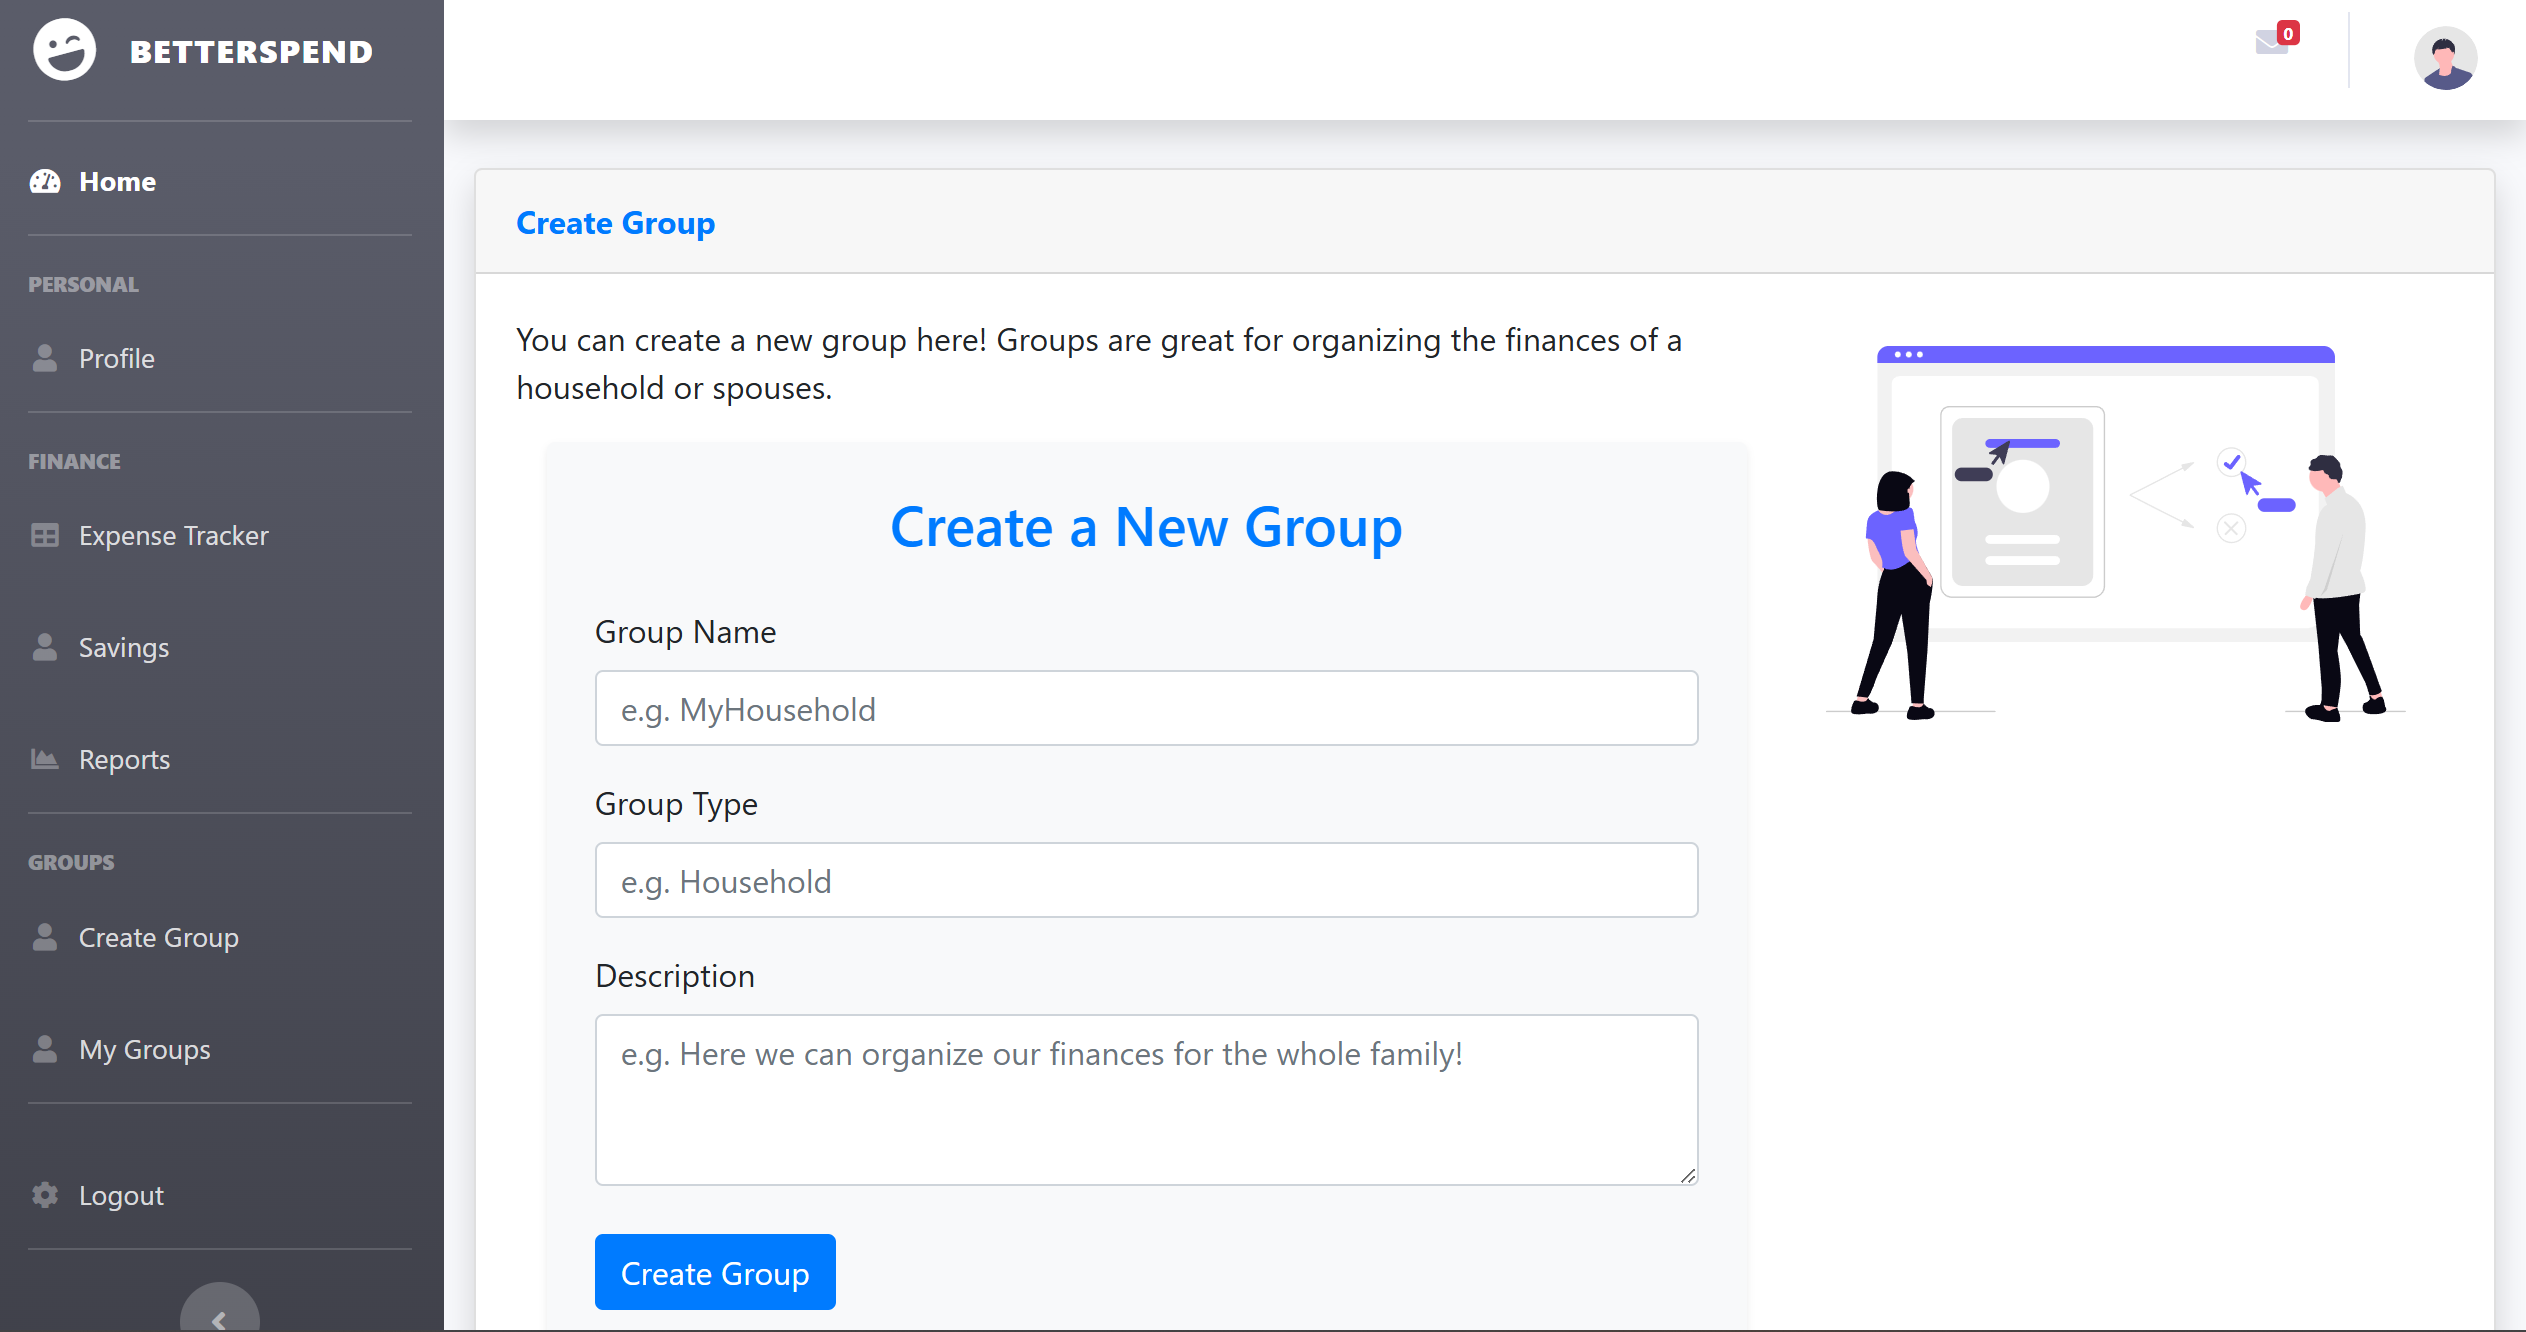
\includegraphics[height=190px]{img/create-group}
	\caption{Screenshot: Create Group oldal}
	\label{fig:create-group}
\end{figure}

\subsubsection{Saját csoportok}
\begin{itemize}
	\item[\emph{Megtekintés}]	 Az \ref{fig:group}. ábrán látható felület a baloldali menüsávból érhető el ("My Groups" menüpont). Az oldalon belül minden csoport külön lapokon tekinthető meg, ezek között lehet navigálni az oldal tetején lévő gombok segítségével. Minden gomb felirata az adott csoport neve. A lapok tetején láthatóak az alap adatok, mint a csoport neve, leírása, tagok és a felhasználó szerepköre ("Admin" = ha ő hozta létre, "Member" = azaz "tag", ha a felhasználó csak meghívva lett a csoportba)
	\begin{figure}[H]
		\centering
		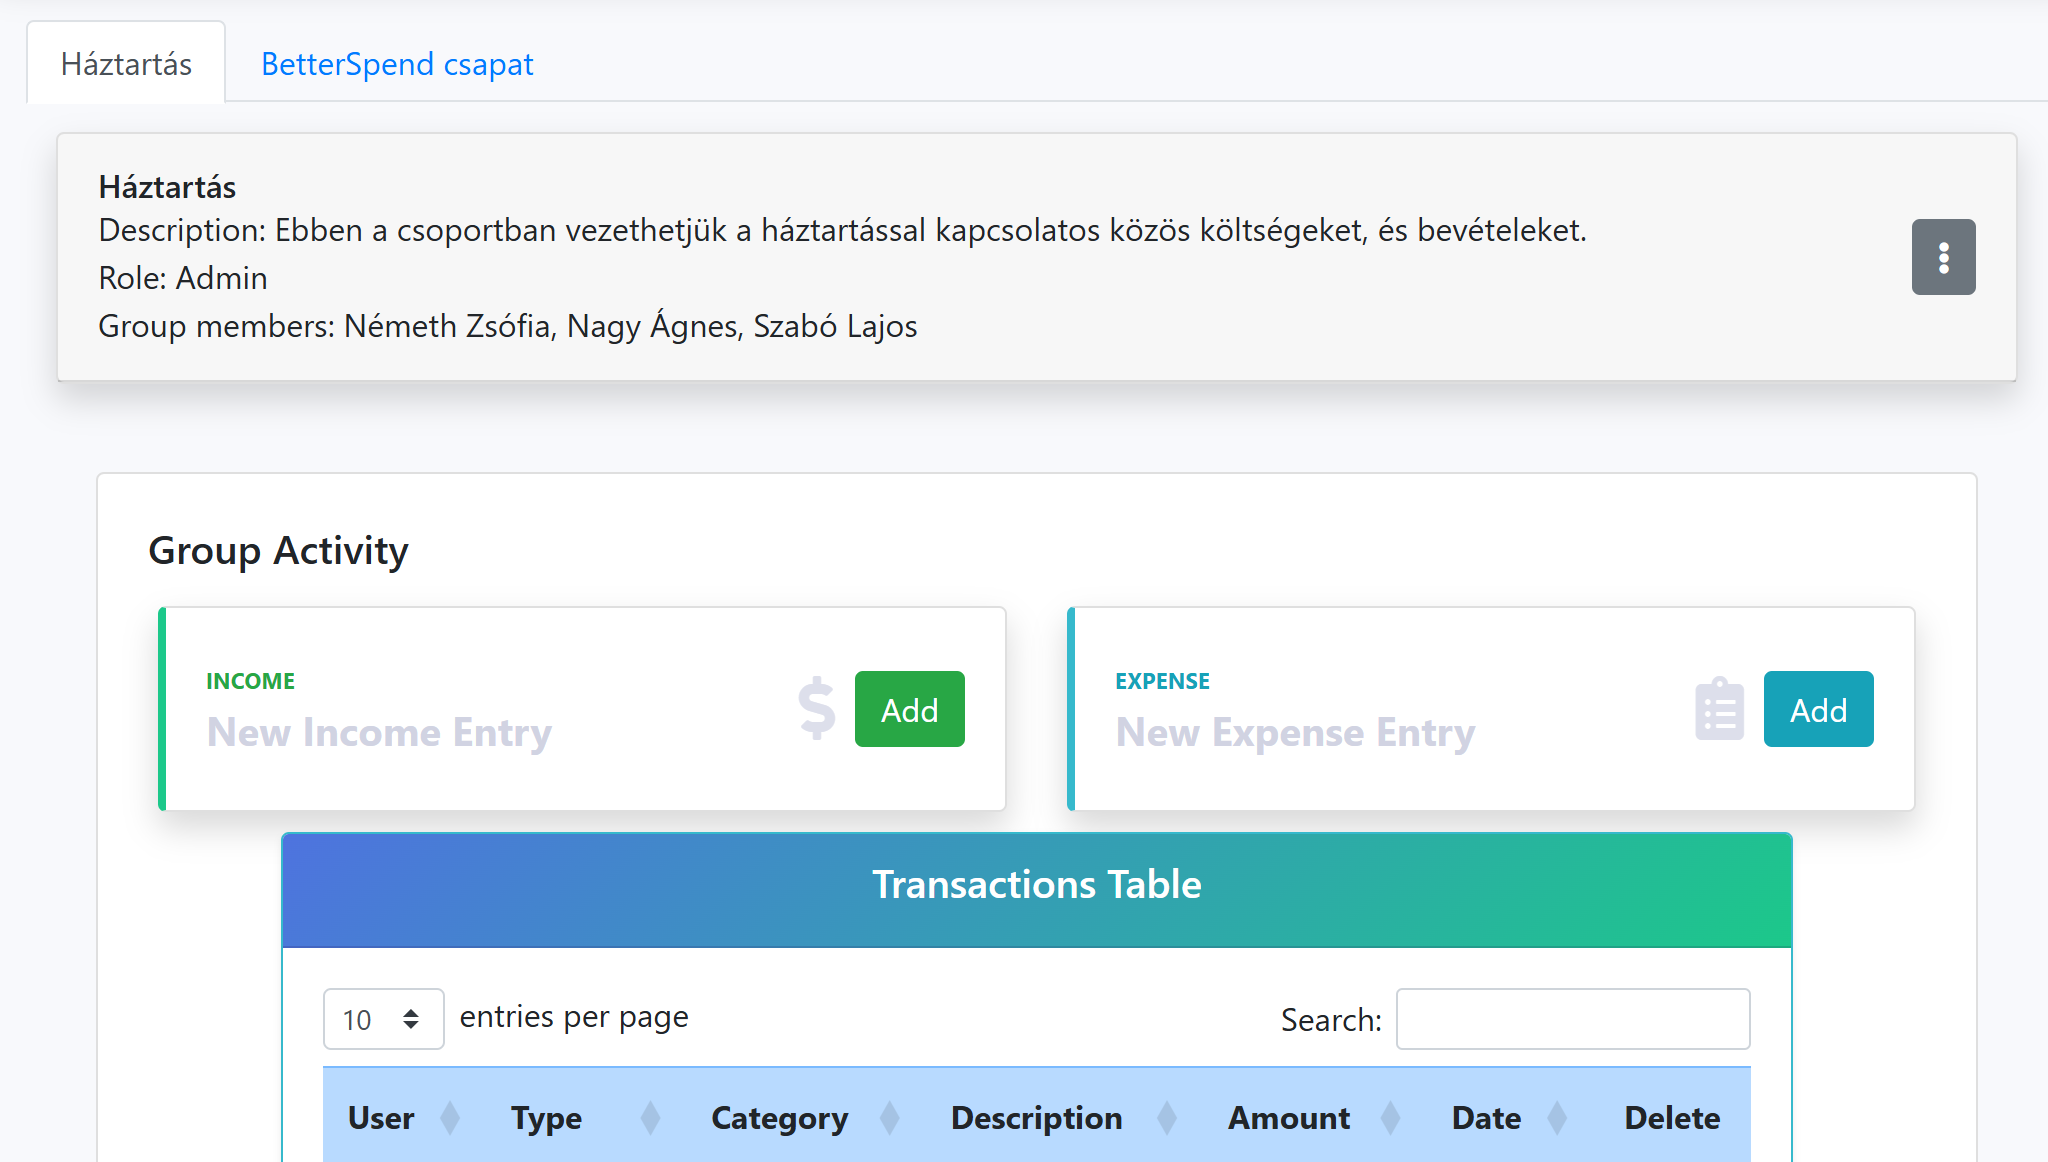
\includegraphics[height=190px]{img/group}
		\caption{Screenshot: My Group oldal}
		\label{fig:group}
	\end{figure}
		\item[\emph{Funkciók}] A csoportos funkciók megegyeznek a személyes funkciókkal (bevételek/kiadások rögzítése és törlése, előzmények megtekintése, megtakarítások létrehozása és kezelése). Ezek részletes bemutatásra már megtörtént korábbi fejezetekben.
	\item[\emph{Kezelés}] Egy adott csoport fejlécének jobb oldalán található 3 pont megnyomása egy leugró menüt nyit meg. Itt lehet meghívót küldeni a csoportba egy másik felhasználónak ("Add member"), elhagyni a csoportot ("Leave group"), vagy ha Admin szerepkörrel rendelkezik az adott felhasználó akkor törölni is lehet a csoportot.
	\begin{figure}[H]
		\centering
		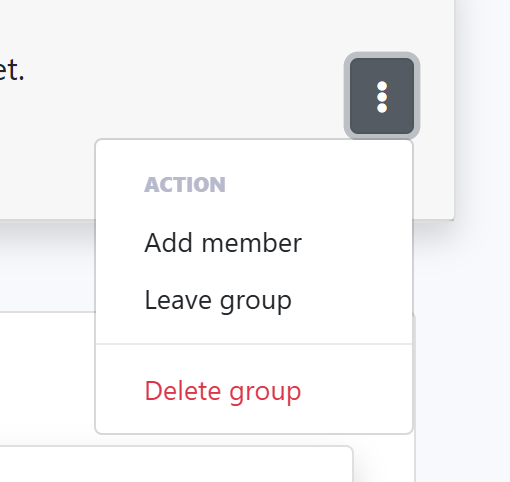
\includegraphics[height=120px]{img/group-actions}
		\caption{Screenshot: Screenshot: Csoport műveletek}
		\label{fig:group-actions}
	\end{figure}
	\item[\emph{Meghívó}] A meghívó küldése után a meghívott felhasználónak érkezni fog egy értesítése (mely az oldal tetején lévő levél ikon megnyomásával válik láthatóvá), amely tartalmazza a következő információkat: csoport neve, felhasználó teljes neve, aki meghívta oda. Itt az \ref{fig:notification} ábrán látható módon egy "Accept" (elfogadás) és egy "Deny" (elutasítás) gomb található. Ha elfogadja a felhasználó a meghívást, akkor tagja lesz a csoportnak. 
	\begin{figure}[H]
		\centering
		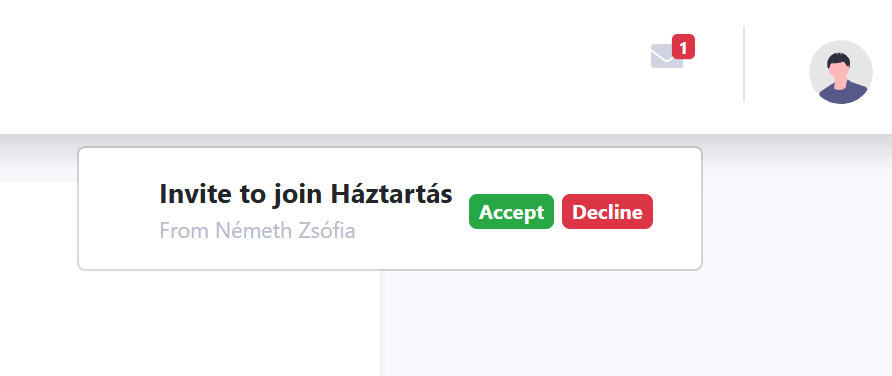
\includegraphics[height=120px]{img/invite}
		\caption{Screenshot: Értesítések}
		\label{fig:notification}
	\end{figure}
\end{itemize}